% !TEX root = ../thesis.tex
\chapter{Návrh a realizace úprav ASR}
\label{chap:realisation}

Experimenty provedené v části \ref{chap:construction:results} jasně ukázaly, že individuální ASR modely jsou relativně obstojně zvládají rozpoznávat EL řeč. individuální a obecné modely pro zdravého řečníka však dosahují významně lepších výsledků. Z experimentu s redukcí fonetické sady (viz část \ref{chap:construction:results:reduction}) vyvstala potřeba rozšířit řečový korpus o příklady promluv obsahující slova mající rozdílný význam, ale lišící se pouze ve znělosti jednoho fonému.

Toto rozšíření totiž umožní lepší porozumnění problematice znělosti EL řeči a pomůže s návrhem úprav akustického modelu tak, aby výsledná přesnost se co možná nejvíce maximalizovala.

%Z experimentů provedených v části \ref{chap:construction:results} vyplynula
%potřeba rozšířit řečový korpus. V části \ref{chap:construction:results:reduction} se ukázalo, že v určitých případech jsou neznělé fonémy produkovány jako znělé. Pro lepší porozumnění tohoto jevu je nezbytné, aby řecový korpus obsahoval co možná nejvíce promluv zahrnující slova s odlišným významem, ale lišící se pouze ve znělosti právě jedonho fonému.x

%Tato část se zaměřuje na získání takovýchto slov a experimentů s nimi. Hlavním experimentem je porovnání schopností člověka a stroje tato slova od sebe odlišit. Na základě poznatků z tohoto experimentu jsou navrženy úpravy, které mají sloužit k zlepšení systémů rozpoznávání řeči.

% Nejprve je v částu \ref{chap:realisation:corpus} popsán proces výběru a získání inkriminovaných slov a následně jsou tato nová data analyzována. V následující části \ref{chap:realisation:test:quality} jsou provedeny kontrolní experimenty, při kterých je zjištěn problém s přenosovým kanálem a na základě těchto zjištění je navrženo řešení. Zbylé dvě části (\ref{chap:realisation:test:listening} a \ref{chap:realisation:test:comparison}) se pak zabývají porovnáním výsledků člověka a stroje na nových datech.

% !TEX root = ../../autoreferat.tex
\section{Vytvoření řečového korpusu EL promluv}
\label{chap:construction:corpus}

% Před započetím prací na vytvoření ASR systému pracujícího s~lidmi po TL je potřeba vytvořit řečový korpus, který poslouží  k~natrénování a otestování vytvořeného systému. Tato data jsou velmi specifická. Proto je potřeba zajistit co možná největší množství kvalitních\footnote{Kvalitou je myšlena věrnost dat dané doméně, dále se mluví o přesnosti ve smyslu bezchybnosti přepisů.} a přesných dat, která budou součástí řečového korpusu.

% Jak už bylo zmíněno v~části \ref{chap:cause:desease}, ročně se objeví více než 100 nových případů trvalé ztráty hlasu, přičemž rizikovou skupinou osob jsou starší lidé, kteří intenzivně kouří a konzumují alkohol. Přesto je patrný trend snižujícího se věku pacientů a s~tím související nárůst případů ztráty hlasu. Přičteme-li již výše zmíněný psychologický aspekt jeho ztráty, je zřejmé, jak komplikované je zajistit spolupráci byť s~jediným řečníkem ochotným podstoupit náročné\footnote{I pro zdravého člověka je někdy několikahodinové nahrávání vysilující. Pro jedince po TL to je z mnoha důvodů ještě řádově náročnější.} nahrávání.

% Proto došlo  k~navázání kontaktů se specializovanými pracovišti ORL, v~našem případě byly nejprve navázány kontakty s~ORL klinikou při Fakultní nemocnici v~Plzni, a následně i s~ORL klinikou Fakultní nemocnice v~Motole.
S pomocí lékařů ORL kliniky při Fakultní nemocnici v~Plzni byla navázána spolupráce s~jedním řečníkem, konkrétně se jedná o dámu v~důchodovém věku, která podstoupila TL před více než 15 lety.
% Po překonání ostychu\footnote{Podle jejích vlastních slov nebyla schopna několik let po operaci ani zvednout nečekaný telefonní hovor, natož mluvit na veřejnosti.} se byla schopna naplno vrátit do běžného života a dokonce v~určité formě opět přednášet o stomatologii na Lékařské fakultě v~Plzni, Univerzity Karlovy.
S její pomocí bylo na pracovišti Katedry kybernetiky ZČU v~1.~etapě nahrávání,
% v~období od prosince 2010 do května 2011,
pořízeno více než 10 hodin promluv.
% během 14 samostatných sezení více než 10 hodin promluv, viz tab. \ref{tab:construction:recording}.
% Každé sezení trvalo přibližně dvě hodiny a bylo rozděleno na fáze nahrávání a fáze odpočinku. Fáze nahrávání trvaly 10 - 20 minut.
Pořízené dílčí nahrávky obsahují několik vět, které jsou vzájemně odděleny úseky ticha o minimální délce 5~s.
% Fáze odpočinku mezi nahráváním dílčích segmentů trvaly přibližně 10 minut.
% Bylo nezbytné je do harmonogramu zařadit zejména z~důvodu únavy řečníka.
Získaná data neobsahují žádný nežádoucí ruch kromě samotného zvuku EL i přesto, že nahrávání neprobíhalo v~profesionálním studiu.

% \begin{table}[htpb]
%   \centering
%   \def\arraystretch{1.5}
%   \pgfplotstabletypeset[
%     col sep=comma,
%     string type,
%     columns/phase/.style={column name={Nahrávání}, column type={l}},
%     columns/length/.style={column name={Délka \textit{[HH:MM:SS]}}, column type={r}},
%     columns/sentences/.style={column name={Počet vět}, column type={r}},
%     columns/files/.style={column name={Počet souborů}, column type={r}},
%     every head row/.style={
%       after row={
%         \cmidrule(r){1-1}
%         \cmidrule(lr){2-2}
%         \cmidrule(lr){3-3}
%         \cmidrule(l){4-4}
%       },
%       before row={\toprule}
%     },
%     every last row/.style={after row={\bottomrule}},
%   ]{./parts/ch5-construction/tabs/02-recording1-stats.csv}
%   \caption{Informace o korpusu nahrávek z 1. etapy nahrávání.}
%   \label{tab:construction:recording}
% \end{table}

Pro pořízení záznamů byla navržena nahrávací sestava složená z miniaturního profesionálního mikrofonu (DPA d:screet 4061-FM), zesilovače (DPA MMA6000), externí zvukové karty a běžného notebooku. Mikrofon byl pomocí bezpolštářkové náplasti přilepen co nejblíže (do bezprostřední blízkosti) pravého koutku úst mluvčí tak, aby zaznamenaná řeč měla co možná nejvyšší kvalitu.

Před samotným nahrávánám byly z databáze obsahující stovky tisíc vět pečlivě vybrány, postupem popsaným v~\cite{Radova2000}, konkrétní věty a z nich vytvořeny 2 sady vět, konkrétně:

\begin{enumerate}
  \item sada obsahující všechny fonémy vyskytující se v~češtině - \textit{40 vět};
  \item sada obsahující věty s~reálnou četností fonémů - \textit{5000 vět}.
\end{enumerate}

% \noindent Nahrané soubory vždy obsahují několik vět vzájemně oddělených minimálně 5 sekundovými úseky ticha.
% Nahrávky mouhou navíc obsahovat opakování chybně vyslovených vět, přeřeknutí, kýchnutí a další neřečové události.
% Z tohoto důvodu bylo nezbytné nahrávky rozčlenit na kratší úseky a anotovat, přestože byly pořízené na základě připravené sady vět.

Každá nahrávka je automaticky rozdělena na mikrosegmenty o konzistentní době trvání. Empiricky byla stanovena vhodná délka trvání v~rozsahu 10 - 100 ms. S~využitím metody voice activity detection (VAD) byla pro každou nahrávku stanovena hodnota energie dle vztahu

\begin{equation}
  \label{eq:construction:energy}
  E_{RMS}(n) = \sqrt{\frac{1}{N} \sum_{n=1}^{N} \left| x(n) \right|^2},
\end{equation}

\noindent kde $N$ představuje počet vzorků v~nahrávce a $x(n)$ představuje pravoúhlé okénko vzorku $n$ a následně určena průměrná energie nahrávky jako střední hodnota energií všech mikrosegmentů.
Její hodnota slouží pro nalezení úseků ticha, tj. míst, kde začíná a končí věta.
Pokud energie nějakého úseku $x$ je $E_{RMS}(x) < avg(E_{RMS})$ a zároveň délka tohoto úseku $dur(x) \geq 1\ s$, tak je možné nahrávku v~tomto úseku rozdělit.
% Na začátku a konci každého úseku je vhodné mít minimálně $0.5\ s$ ticha, aby byla zajištěna správná funkce ASR systému, viz \ref{chap:asr:parametrization}.
Na obr. \ref{fig:construction:el_speech} je zobrazena ukázka charakteru audio signálu a spektrogram promluvy \textit{\uv{Akcie Komerční banky}}.
% Zároveň jsou zde vyneseny vypočtené hodnoty energie a celková průměrná energie.
% Pokud řečník v~průběhu věty z~libovolného důvodu udělal pauzu větší než $1\ s$, tak i tato věta byla v~důsledku výše popsaného postupu rozdělena na dvě části.
% Nejedná se však o významný problém, protože při vytváření ASR systému není podstatné, zda promluva představuje celou větu, ale spíše to, zda je tento úsek správně přepsán.
% Fakt, že některé věty jsou rozděleny na více částí, je důvodem, proč v~tab. \ref{tab:construction:recording} neodpovídá počet soubourů počtu vět.

\begin{figure}[hbpt]
  \centering
  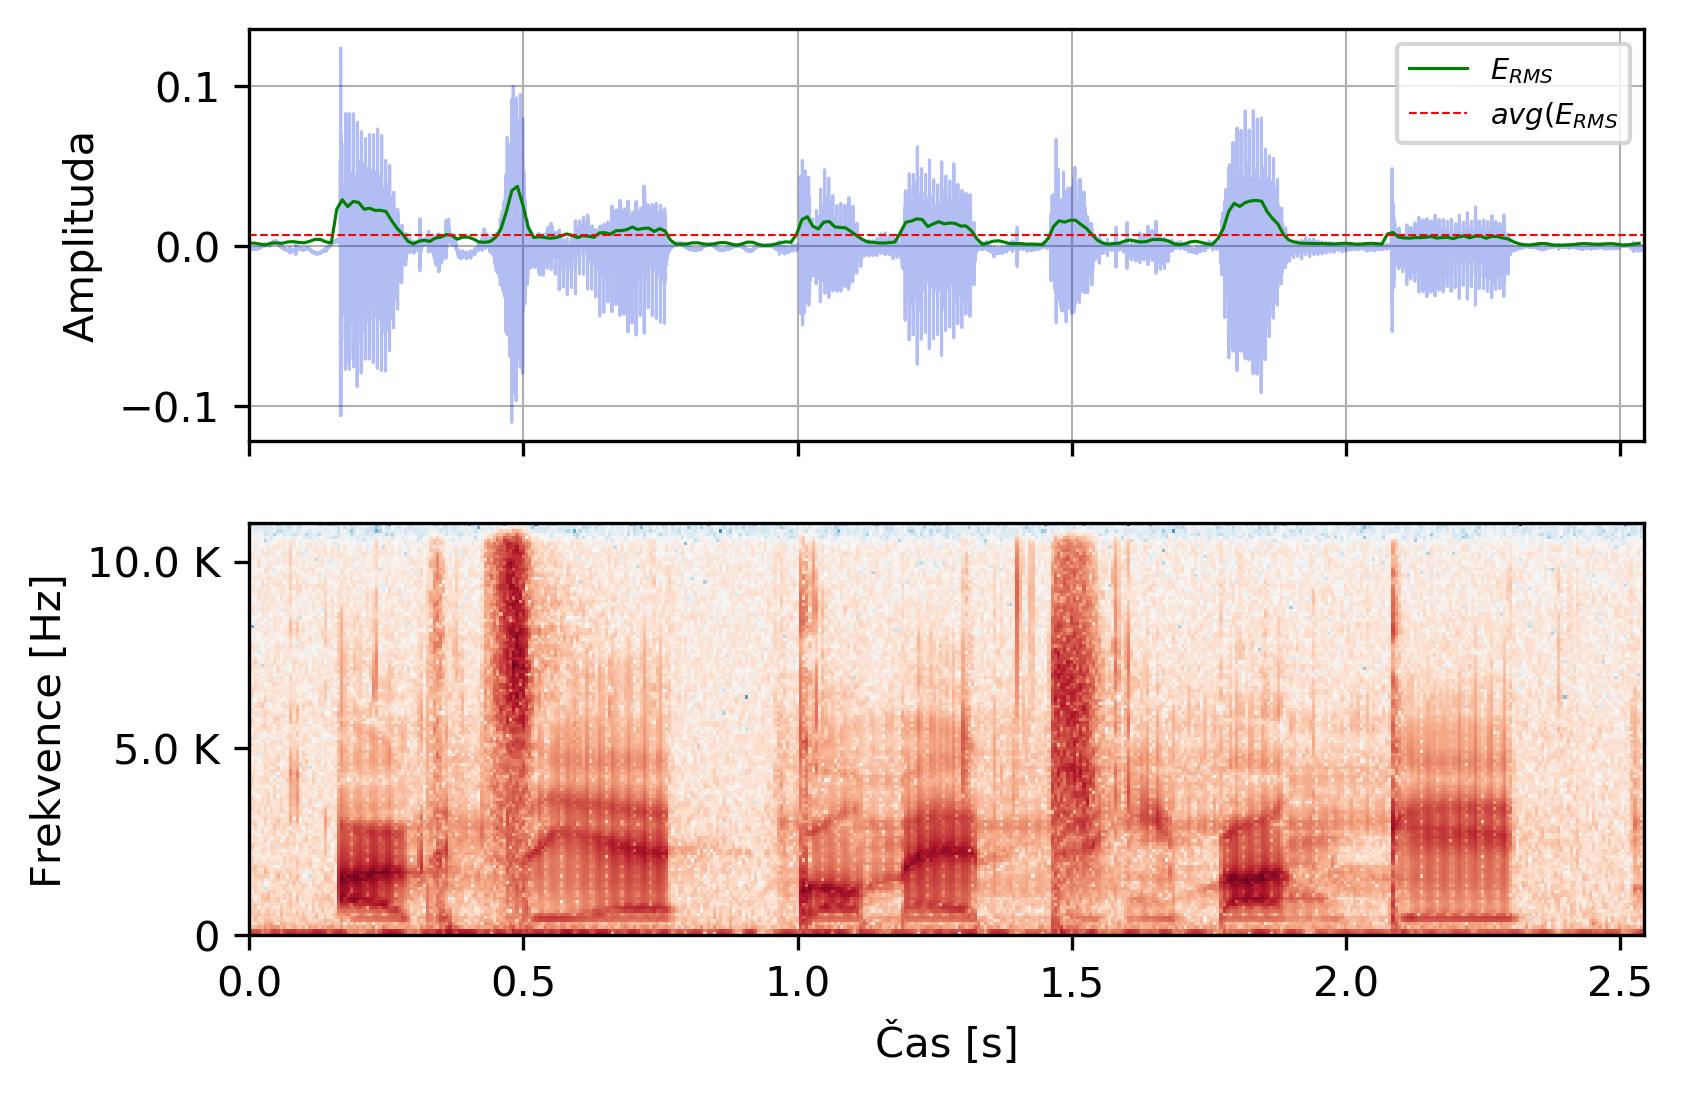
\includegraphics[width=0.9\textwidth]{./parts/ch5-construction/img/energy_spec_el.png}
  \caption[Průběh a spektrogram EL promluvy.]{Průběh a spektrogram promluvy a vyznačenou energií EL promluvy.}
  \label{fig:construction:el_speech}
\end{figure}

% K anotaci posloužil interní anotační nástroj, podíleli se na ní celkem 3 anotátoři z~řad studentů.
% Přepis každého anotátora byl vždy zkontrolován jiným anotátorem.
% Ačkoli bylo potřeba přepsat relativně malé množství dat (cca 10 hodin audio záznamu), tak anotace všech promluv trvala přibližně 2 měsíce.
% Hlavním důvodem byla relativně dlouhá doba, po kterou se anotátoři adaptovali na specifika EL řeči.
% Hlavně ze začátku nebyli schopni porozumět obsahu promluvy, a tím pádem jej správně přepsat.
% To významně prodloužilo dobu potřebnou  k~anotaci celého řečového korpusu.

% Pokud je  k~produkci řeči použit elektrolarynx, je vedlejším produktem nezanedbatelný ruch způsobený samotným zařízením, viz část \ref{chap:cause:treatment:foniatric}.
% Z~tohoto důvodu byly v~průběhu anotace ignorovány v~podstatě všechny skupiny neřečových událostí, protože vetšina nahrávek by dle pravidel anotování běžné řeči obsahovala šum.
% Výsledný řečový korpus se skládá z $5040$ unikátních vět rozdělených do $6385$ souborů (viz tab. \ref{tab:construction:recording}), které v~průměru obsahují $7$ slov o průměrné délce $5$ znaků. Tento korpus slouží jako základ pro všechny budoucí experimenty.

% !TEX root = ../thesis.tex
\section{Poslechový test a porovnání výsledků člověka a stroje}
\label{chap:realisation:listening}

V předchozím textu byly prezentovány vybrané dosažené výsledky, ale ty zatím nedokázaly odpovědět na zásadní otázku: \uv{Dokáže se stroj\footnote{Stroj je reprezentován systémem automatického rozpoznávání řeči.} vyrovnat človéku?}.
Přestože je EL řeč na první poslech obtížně srozumitelná, tak již po krátké době je člověk schopen obstojně rozumět.
S přibývajícím časem se do určité míry porozumění ještě zlepšuje.
Jak je na tom tedy stroj v~porovnání s~člověkem?

Ještě než je vůbec možné na tuto otázku odpovědět, tak je dobré si odpovědět na otázku: \uv{Jakým způsobem porovnat schopnosti člověka a stroje?}.
K tomu může posloužit poslechový test, ve kterém mají posluchači za úkol vybrat z předem definovaných možností, co je obsahem promluv.
Otestování schopností stroje pak probíhá pomocí experimentu.
Vstupem ASR systému jsou stejné promluvy, které jsou součástí poslechového testu.
Výstupem je přepis.
Metrika experimentu je počítána na základě správně/špatně určeného obsahu promluv v~přepisu\footnote{Výstup ASR systému je považován za správný i v~případě, že se liší např. i/y. Z akustického pohledu jsou totiž oba fonémy identické.}.
Prostým porovnáním počtu správných odpovědí člověka a stroje je možné odpovědět na první z výše uvedených otázek.

Při přípravě experimentu vykrystalizovaly tyto varianty poslechového testu:

\begin{itemize}
  \item test na izolovaných slovech,
  \item test na slovních bigramech (dvojicích slov).
\end{itemize}

\noindent Tím, že promluvy obsahují pouze izolovaná slova, resp. dvojici slov je do značné míry eliminován vliv kontextu.
Ten v~mnoha případech pomáhá se správným určením významu i přesto, že nebylo dobře rozumět.
Pokud se bude experiment skládat z~množiny promluv, které obsahují pouze slova popsaná v~části \ref{chap:realisation:corpus}, tak bude možné určit, do jaké míry dokáže člověk, resp. stroj správně určit význam těchto slov a případně je od sebe odlišit.

\subsection{Izolovaná slova}
\label{chap:realisation:listening:isolated}

Rozpoznání slova, které bylo vysloveno v~klidném prostředí se jeví jako velice jednoduchý úkol.
Pokud jej ale vyslovil řečník používající EL, tak už to tak snadné být nemusí.
Zvlášť pokud se jedná o slova popsaná v~\ref{chap:realisation:corpus}.
Účastníci poslechového testu na izolovaných slovech mají za úkol postupně vyslechnout $320$ nahrávek izolovaných slov a vybrat jednu z předem definovaných odpovědí:

\begin{enumerate}[label=\alph*)]
  \item slovo A \textit{(např. kosa)},
  \item slovo B \textit{(např. koza)},
  \item nemohu rozhodnout.
\end{enumerate}

\noindent Ve výčtu možností je vždy skutečně pronesené slovo a  k~němu pak varianta lišící se pouze znělostí jednoho fonému. První dvě možnosti jsou vždy v~abecedním pořadí. Nahrávky použité v~rámci poslechového testu pocházejí z 2. etapy nahrávání. Poslechového testu se účastnilo $19$ subjektů z řad kolegů.

Výstupy poslechového testu byly vyhodnoceny a zapsány do tabulky s~procentuálním zastoupením jednotlivých odpovědí pro každou nahrávku.
V tab. \ref{tab:realisation:listening:isolated} je ukázán výňatek získaných výsledků. Správné odpovědi jsou zvýrazněny tučně.
Výsledky slov \textit{borce} a \textit{porce} reprezentují situaci, kdy účastník nebyl jednoznačně schopen určit význam slova.
Druhý příklad (\textit{kosa} + \textit{koza}) ukazuje situaci, kdy všichni účastníci vybrali z komplementárních slov vždy pouze jediné, a to nehledě na to, které jim bylo ve skutečnosti puštěno.
V tomto konkrétním případě tedy posluchači vždy \uv{slyšeli} slovo \uv{koza}.
Dalo by se tedy usuzovat, že slova \uv{kosa} je akusticky identické se slovem \uv{koza}.
Poslední případ reprezentuje situaci, kdy byla většina účastníků schopna určit správný význam slova.
Celková přesnost rozpoznávání byla vypočtena podle vzorce

\begin{equation}
  Acc_w^{human} = \frac{1}{N} \sum_{i=1}^{N} f_i * 100,
  \label{eq:realisation:accuracy:human}
\end{equation}

\noindent kde $N=320$ a $f_i$ se rovná relativní četnosti správných odpovědí na otázku $i$ v~poslechovém testu s~izolovanými slovy. Dosáhla hodnoty $Acc_w^{human} = 70,47~\%$.

\begin{table}[htpb]
  \centering
  \def\arraystretch{1.5}
  \pgfplotstabletypeset[
    col sep=semicolon,
    string type,
    columns/word/.style={column name=Slovo, column type={l}},
    columns/option1/.style={
      column name={\textit{\textbf{a)}}},
      column type={r}
    },
    columns/option2/.style={
      column name={\textit{\textbf{b)}}},
      column type={r}
    },
    columns/option3/.style={
      column name={\textit{\textbf{Nevím}}},
      column type={r}
    },
    every head row/.style={
      after row={
        \cmidrule(r){1-1}
        \cmidrule(l){2-4}
        % \midrule
      },
      before row={\toprule & \multicolumn{3}{c}{Relativní četnost odpovědí [\%]} \\}
    },
    every row no 1/.style={after row={
      \cmidrule(r){1-1}
      \cmidrule(l){2-4}
    }},
    every row no 3/.style={after row={
      \cmidrule(r){1-1}
      \cmidrule(l){2-4}
    }},
    every last row/.style={after row={\bottomrule}},
  ]{./ch5-construction/tabs/0206-isolated.csv}
  \caption{Ukázka výsledku poslechového testu na izolovaných slovech.}
  \label{tab:realisation:listening:isolated}
\end{table}

\subsection{Slovní bigramy}
\label{chap:realisation:listening:bigrams}

V druhém poslechovém testu mají posluchači za úkol vyslechnout $333$ nahrávek slovních bigramů\footnote{Nahrávky obsahují dvě po sobě vyslovená slova.} a vybrat jednu z předem definovaných odpovědí. Ty mají vždy tento formát

\begin{enumerate}[label=\alph*)]
  \item slovo A + slovo A \textit{(např. kosa + kosa)},
  \item slovo A + slovo B \textit{(např. kosa + koza)},
  \item slovo B + slovo A \textit{(např. koza + kosa)},
  \item slovo B + slovo B \textit{(např. koza + koza)}.
\end{enumerate}

\noindent Je zřejmé, že to představuje všechny kombinace, které lze z dvojice slov vytvořit. Rozšířený řečový korpus, tak jak je popsaný v~části \ref{chap:realisation:corpus}, ale neobsahuje tento typ nahrávek. Tím pádem je potřeba je vytvořit \uv{uměle}. Což není velký problém, každá nahrávka izolovaného slova obsahuje minimálně $0,5\ s$ ticha na svém začátku a konci. Pokud jsou tyto nahrávky spojeny\footnote{Ke spojení je možné použít nástroj \textit{ffmpeg} nebo \textit{sox}.}, vznikne jediná nahrávka obsahující dvě zájmová slova oddělena krátkou pauzou. Z každé dvojice slov vznikly vždy dvě nahrávky lišící se pořadím slov.

Vyšší počet položek v~testu je zapříčiněn faktem, že pro určitá slova existuje více než jedna kombinace s~jiným slovem\footnote{Ve valné většině se jedná o slova obsahující písmena \textit{i/y}, která jsou v~akustické formě identická. Příkladem může být dvojice \textit{nebyli + nepili} a \textit{nebili + nepili}.}. Ve snaze zkrátit, už tak docela náročný poslechový test, byly vygenerovány bigramy odpovídající pouze možnostem \textit{b)} a \textit{c)}. Účastníci poslechového testu o tom však nebyli informováni. Přesto tento poslechový test dokončilo pouze $12$ účastníků.

Stejně jako u testu s~izolovanými slovy je výstup testu zpracován do tabulky obsahující procentuální zastoupení jednotlivých odpovědí na každou otázku.
Tab. \ref{tab:realisation:listening:bigrams} obsahuje ukázku těchto výsledků.
Stejně jako v~předchozím případě jsou správné odpovědi zvýrazněny tučně.
Ačkoli jsou nyní v~testu dvojice slov, tak dosažené výsledky do značné míry korespondují s~výsledky z testu s~izolovanými slovy (viz tab. \ref{tab:realisation:listening:isolated}).
V~prvním případě (\textit{borci + porci}) nebyli účastníci schopni jednoznačně určit význam slov v~nahrávce.
V~druhém případě (\textit{kosa + koza}) všichni posluchači až na jednoho vybrali možnost \textit{d)}, tedy \textit{koza + koza}.
Správný výběr jedním účastníkem lze považovat spíše za náhodu, protože u opačného pořadí slov již nikdo správnou odpověď nevybral.
Je dobré zmínit, že účastníci v~žádném z provedených poslechových testů nebyli omezeni počtem opětovného přehrání promluvy.
Tím pádem je velmi pravděpodobné, že tento konkrétní participant opakovaně poslouchal danou nahrávku a hledal rozdíl až nějaký drobný zaznamenal.
% Otázkou však je, jestli to spíše nebyla sugesce a to již zmíněné štěstí.

Poslední prezentovaný příklad zastupuje množinu odpovědí, kdy účastníci naprosto správně určili význam slov.
Průměrná dosažená přesnost rozpoznávání člověka, počítána pomocí rovnice (\ref{eq:realisation:accuracy:human}), dosáhla hodnoty $Acc_{w}^{human} = 66,24~\%$.

\begin{table}[htpb]
  \centering
  \def\arraystretch{1.5}
  \pgfplotstabletypeset[
    col sep=semicolon,
    string type,
    columns/word/.style={column name=Slovní bigram, column type={l}},
    columns/option1/.style={column name={\textit{\textbf{a)} A + A}}, column type={r}},
    columns/option2/.style={column name={\textit{\textbf{b)} A + B}}, column type={r}},
    columns/option3/.style={column name={\textit{\textbf{c)} B + A}}, column type={r}},
    columns/option4/.style={column name={\textit{\textbf{d)} B + B}}, column type={r}},
    every head row/.style={
      after row={
        \cmidrule(r){1-1}
        \cmidrule(l){2-5}
        % \midrule
      },
      before row={\toprule & \multicolumn{4}{c}{Relativní četnost odpovědí [\%]} \\}
    },
    every row no 1/.style={after row={
      \cmidrule(r){1-1}
      \cmidrule(l){2-5}
    }},
    every row no 3/.style={after row={
      \cmidrule(r){1-1}
      \cmidrule(l){2-5}
    }},
    every last row/.style={after row={\bottomrule}},
  ]{./ch5-construction/tabs/0207-bigrams.csv}
  \caption{Ukázka výsledku poslechového testu na dvojicích slov.}
  \label{tab:realisation:listening:bigrams}
\end{table}

\subsection{Výsledky porovnání}
\label{chap:realisation:comparison}

Výsledky poslechového testu ukázaly přesnost rozpoznání člověka.
Nyní je potřeba zjistit, jak je na tom stroj zastoupený ASR systémem.
% K tomu je nezbytné natrénovat akustický model a použít vhodný jazykový model.
Byl využit model HMM-DNN, konkrétně se jednalo o DNN síť s~$6$ vrstvami ($5$ skrytých vrstev, každá s~$4096$ neurony), přičemž výstupní vrstva byla typu softmax s~dimenzí rovnou počtu HMM stavů.
Parametrizace byla provedena pomocí PLP (12 kepstrálních koeficientů + delta + delta-delta parametry) a pro eliminaci vlivu kanálu CMN počítané přes všechny nahrávky v~rámci etapy.
Výsledný příznakový vektor má dimenzi $36$.
Vstupem neuronové sítě je parametrizované okénko mající kontext přes $11$ mikrosegmentů, tedy $t-5$ a $t+5$.
Vstupní dimenze neuronové sítě je tedy $396$.
Oproti dosavadním experimentům je v~tomto případě použit vlastní real-time dekodér (více o dekódování v~části \ref{chap:asr:decoding}).
Tento LVCSR systém je optimalizován pro co nejnižší latenci a je schopný pracovat s~velmi velkými slovníky čítající i miliony položek.
Tento dekodér byl vyvinut na Katedře kybernetiky Fakulty aplikovaných věd.

Provedené poslechové testy poskytly dva typy výsledků.
První reprezentuje schopnost určit význam izolovaného slova, druhý schopnost rozeznat dvě velmi podobná slova.
Pro potřeby porovnání přesnosti rozpoznávání člověka s~výsledky dosaženými ASR systémem, byly navrženy celkem $3$ experimenty využívající výše popsaný akustický model.

První experiment odpovídá poslechovému testu s~izolovanými slovy.
Jeho základem je zerogramový LM obsahující více než 1 milion slov.
Většina předchozích experimentů využívala fonémový zerogramový model, aby bylo možné eliminovat vliv LM na výslednou přesnost rozpoznávání.
U těchto experimentů je tento LM nevyhovující, protože cílem je správně určit celé slovo, a proto je využit slovní jazykový model.
U zerogramového modelu mají všechny položky stejnou pravděpodobnost, tím je zaručeno, že nebudou preferována četnější slova.
Slovník potřebný pro tento LM je sestaven z textů pocházejících z novinových článků, webových zpravodajských serverů, filmových titulků a přepisů televizních pořadů.
Využití takto velkého LM vychází z představy, že i člověk má obsáhlou slovní zásobu a dopředu nezná obsah konkrétní promluvy v~rámci testu.
Tento test je pojmenován jako \uv{one-mil}.

Ve skutečnosti však účastníci znají seznam slov zahrnutých do poslechového testu a mají tak určitou výhodu oproti \uv{one-mil} nastavení.
Za účelem kompenzace tohoto vlivu, je vytvořen druhý experiment, který pracuje s~redukovaným LM.
Obsahuje pouze slova, která se opravdu vyskytla v~rámci poslechového testu ($N = 320$).
Tento experiment je nazván jako \uv{reduced}.
Výsledky obou těchto experimentů byly porovnány s~poslechovým testem na izolovaných slovech.
Další možností by mohlo být vytvoření speciálních LM pro každou promluvu.
Ten by obsahoval pouze komplementární slova.
Problémem tohoto postupu je třetí možnost, kterou obsahuje poslechový test (tzv. \uv{nemohu rozhodnout}).
V případě, že by LM obsahoval pouze dvě slova, tak by ASR experiment, svými parametry, neodpovídal poslechovému testu.

Poslední navržený experiment spočívá v~tom, že je ke každé nahrávce se slovním bigramem vygenerován speciální (zerogramový) LM.
Ten obsahuje vždy pouze všechny 4 kombinace slov.
Tím pádem odpovídá dostupným možnostem v~rámci poslechového testu.
Tento experiment je nazván jako \uv{bigrams}.
Jeho výsledky jsou porovnány s~druhým poslechovým testem.

Výsledkem rozpoznávače je nejlepší hypotéza (případně \textit{N} nejlepších hypotéz), tudíž slovo.
To však není porovnatelné s~výsledkem poslechového testu.
Z tohoto důvodu jsou všechny výsledky ohodnoceny $1$, pokud bylo výstupem správné slovo, a v~opačném případě $0$.
Násladně byl z tohoto ohodnocení vypočten průměr.
Pro upřesnění je nutné zmínit, že \textit{i/y} na výsledném ohodnocení nehraje roli.
Dosažené výsledky jsou pak shrnuty v~tab. \ref{tab:realisation:comparison}.
Ty ukazují, že řešení takového úkolu je výzvou nejen pro člověka, ale i pro stroj.
V případě experimentu \uv{one-mil} je úspěšnost rozpoznávání ASR systému významně nižší než úspěšnost rozpoznání člověka.
To je způsobeno především enormní perplexitou jazykového modelu.
Ta je rovna velikosti slovníku.
Po zmenšení slovníku se podařilo získat výsledky srovnatelné s~člověkem.
Je ale potřeba zdůraznit, že i v~případě \uv{reduced} experimentu vykazuje člověk vyšší úspěšnost rozpoznání, protože čelí pouze perplexitě $3$ (kdykoli může podívat na nabízené možnosti).
Tento faktor by bylo možno eliminovat tak, že by účastník testu přepsal obsah promluvy a tento přepis by byl následně porovnán se skutečným obsahem.
To by ale významně zvýšilo časovou náročnost poslechového testu a bylo by velmi komplivané získat kompletní výsledky od relevantního množství účastníků.
Už jen podíl odpadlíků mezi prvním a druhým poslechovým testem dosáhl závratných $30~\%$.

Velmi zajímavé jsou výsledky u~\uv{bigrams} experimentu.
Na první pohled se může jevit jako snazší, protože úkolem je vybrat z jasně definovaných kombinací slov.
Slova jsou si ale akusticky velmi podobná a v~mnoha případech je velmi náročné je od sebe rozeznat.
Jak člověk, tak stroj, dosáhli v~tomto testu nejhorších výsledků.
Při analýze se ukázalo, že rozdíly mezi hypotézami ASR systému jsou velmi malé, což naznačuje velkou podobnost mezi inkriminovanými modely fonémů.
Zároveň tyto výsledky s~velmi podobnými hypotézami korelují s~výsledky poslechového testu, kde posluchači nebyli schopni jednoznačně rozhodnout o významu jednotlivých slov.

\begin{table}[htpb]
  \centering
  \def\arraystretch{1.5}
  \pgfplotstabletypeset[
    col sep=semicolon,
    string type,
    columns/type/.style={column name= , column type={l}},
    columns/onemil/.style={column name={one-mil}, column type={r}},
    columns/reduced/.style={column name={reduced}, column type={r}},
    columns/bigrams/.style={column name={bigrams}, column type={r}},
    every head row/.style={
      after row={
        % \cmidrule(lr){1-1}
        % \cmidrule(lr){2-4}
        \midrule
      },
      before row={\toprule & \multicolumn{3}{c}{$Acc\ [\%]$} \\}
    },
    every last row/.style={
      after row={\bottomrule}
    },
  ]{./ch5-construction/tabs/0208-comparison.csv}
  \caption{Porovnání dosažených výsledků člověka a stroje.}
  \label{tab:realisation:comparison}
\end{table}

Na základě dosažených výsledků lze tvrdit, že stroj prozatím nedosahuje schopností člověka.
Pokud uvážíme, že byl člověk oproti stroji vždy v~malé výhodě, tak dosažené výsledky jsou relativně optimistické.
Minimálně v~jednom případě se stroj téměř vyrovnal člověku.
Samotnou kapitolou je vliv slovního kontextu.
Ještě před samotnými experimenty byl ověřen výkon ASR systému na \uv{kontinuální} řeči, zde reprezentované pomocí vět z testovací sady.
Jazykovým modelem je v~tomto případě trigramový slovní model obsahující $1,2$ milionu unikátních slov.
Přesnost rozpoznávání na slovech (počítaná pomocí rovnice (\ref{eq:asr:decoding:acc})) dosáhla hodnoty $86,10~\%$.
Při porovnání této hodnoty s~výsledky uvedenými v~tab. \ref{tab:realisation:comparison} lze konstatovat, že pokud je k~dispozici dostatečný kontext, tak je ASR schopen lépe určit variantu slova.
Přeci jen slovo \uv{kosa} se většinou vyskytuje v~trochu jiném slovním kontextu, než slovo \uv{koza}, a toto platí u většiny dvojic.

% !TEX root = ../../autoreferat.tex
\section{Augmentace dat}
\label{chap:realisation:augmentation}

% Poslechový test jasně ukázal, že správné rozpoznání pronesené EL promluvy není lehký úkol ani pro člověka.
Naprosto markantní význam má kontext.
% Ten pomáhá v~případě, že některým částem promluvy nebylo dobře rozumět.
% Navíc, ze zkušeností získaných při pořizování řečového korpusu (části \ref{chap:construction:corpus} a \ref{chap:realisation:corpus}) plyne, že EL řečník má tendenci mluvit ve spíše kratších dávkách slov, mezi kterými dělá drobné pauzy.
% Pro člověka není problém udržet v~povědomí kontext, ale stroji to může někdy způsobovat problémy.
% Otázkou tedy je, jak \uv{vylepšit} stroj tak, aby poskytoval lepší výsledky.

Ať se řečník snaží sebevíc, tak i při využití metod rehabilitace hlasu uvedených v~části \ref{chap:cause:treatment}, se v~důsledku ztráty hlasivek část informace z produkované řeči ztrácí.
V poslední době bylo prezentováno několik přístupů jak ztracenou informaci obnovit.
Souhrn těch nejperspektivnějších je v~\cite{Denby2010}.
Ve valné většině případů se využívá obohacení akustického modelu o artikulační data, nebo dokonce využití jen těchto artikulačních dat \cite{Hofe2013} .
Problém ale spočívá v~tom, že ne všechny akustické nuance mezi podobnými fonémy jsou artikulací ovlivněny.
Pořízení záznamu artikulačních dat často vyžaduje používaní dalšího zařízení (kamery, ultrazvuku, atp. \cite{Hueber2010, Fagan2008, Jorgensen2010, Hirahara2010},
nebo dokonce nutnost podstoupení dalšího operačního zákroku (magnety \cite{Hofe2011}).
Samozřejmě je nutno říct, že většina těchto vyvíjených systémů si klade za cíl kompletně nahradit současné metody rehabilitace hlasu.
Na druhou stranu faktem je, že ani po dlouholetém vývoji se většina těchto systémů nedostala z~rané vývojové fáze.
Nepochybně hraje roli i skutečnost, že tato problematika není v~ohnisku zájmu řečařské komunity.

Pokud tedy není úplně reálné získat ztracenou informaci pomocí kompletní změny paradigmatu fungování systémů rozpoznávání řeči, tak zbývá jen pracovat s~informací, která je  k~dispozici, a adaptovat současný model.
Určitou možností je nahrazení ztracené informace konkrétní cílenou změnou produkované řeči,
která je zohledněna modelem.
Samozřejmě takovýto přístup nezbaví řečníka elektrolarynxu, ale může mu pomoci v~situacích, které jsou pro něj stresující a~v konečném důsledku mu velmi komplikují život.

% Jako nejjednodušší možnost augmentace se jeví protažení určitých fonémů.
% Člověk je naprosto bez problémů schopen měnit tempo promluvy.
% Dokonce se tato změna velmi často děje mimoděk, protože tempo řeči velmi významně závisí na emočním a fyzickém stavu jedince.
% Pokud by se řečník naučil automaticky protahovat určité fonémy, teoreticky by to mohlo pomoci při rozpoznávání.
% U HMM modelů se délka fonému modeluje pomocí přechodu ze stavu $s_x$ do stejného stavu $s_x$, viz kapitola \ref{chap:asr:acoustic:HMM}.
% Z výsledků poskytnutých \uv{bigrams} experimentem (část \ref{chap:realisation:listening:bigrams}) se dá usuzovat, že modely fonémových párů lišících se znělostí jsou si velmi podobné.
% Protažení jednoho fonému z inkriminovaného páru může vést  k~lepšímu odlišení těchto modelů, a tím pádem i k~vyšší přesnosti rozpoznávání.

% K ověření jsou potřeba data.
Bohužel získání reálných dat je časově náročný proces (viz \ref{chap:construction:corpus} a \ref{chap:realisation:corpus}).
Navíc není zřejmé, jestli se vůbec vyplatí taková data pořizovat, protože se jedná o hypotézu.
Mnohem snadněji se jeví pro účely testování možnost uměle data protáhnout v~místech výskytu zájmových fonémů.
Toto protažení je teoreticky možné realizovat dvěma způsoby:

\begin{enumerate}
  \item protažením na příznacích;
  \item protažením na zvuku.
\end{enumerate}

\noindent V~obou případech je nezbytné získat co možná nejpřesnější fonetické zarovnání. Pokud bude obsahovat chyby, tak mohou být protahovány úplně jiné úseky řeči. K~natrénování HMM-DNN modelu na protažených datech je zapotřebí zarovnání získané HMM-GMM nebo HMM-DNN modelem, viz \ref{chap:asr:acoustic:DNN}. U obou variant protažení je postup stejný:

\begin{enumerate}
  \item natrénování akustického modelu na originálních datech;
  \item získání zarovnání;
  \item protažení zájmových fonémů podle zarovnání;
  \item natrénování nového akustického modelu na protažených datech.
\end{enumerate}

\noindent Nový model může být otestován a získané výsledky mohou být porovnány s~těmi dosavadními.
Tyto experimenty navíc pomohou určit vhodné hodnoty parametrů pro případné skutečné protažení dat.

\subsection{Protažení na příznacích}
\label{chap:realisation:augmentation:features}

Protažení na příznacích je založeno na skutečnosti, že při protažení (např. fonému) a následné parametrizaci, budou v~inkriminovaných mikrosegmentech po sobě následovat velmi podobné příznakové vektory.
% Teoreticky by v~krajním případě mohlo dojít i  k~situaci, kdy část těchto příznakových vektorů bude identických.
% Pokud bude cílem zjistit, zda protažení může pomoci při rozpoznávání EL řeči, tak je možné (teoreticky) docílit protažení zkopírováním určitých příznakových vektorů.
% Tato myšlenka je přiblížena na obr. \ref{fig:realisation:augmentation:features}.
V prvním kroku je nahrávka standardně parametrizována.
% Barevně jsou vyznačeny případné vektory odpovídající zájmovému úseku (tedy fonému).
% Konkrétní hranice jsou získány ze zarovnání.
Tyto vektory jsou následně zduplikovány a představují dvojnásobné protažení.
% V reálné situaci by řečník mluvil jako doposud a k~protažení by docházelo až při zpracování, což je velmi netriviální úkol.
% Teoreticky by musel algoritmus parametrizace být doplněn o mechanismus, který by určité příznakové vektory definovaným způsobem duplikoval.
% Problém je, že by ke kopírování docházelo v~momentě předzpracování, kdy jsou o daných příznakových vektorech k~dispozici minimální informace.
% Prosté zkopírování navíc narušuje dynamický charakter řeči.
% V rámci jednoho zpracovávaného mikrosegmentu jsou parametry považovány za statické, ale jak se okénko v~rámci zpracování posouvá, tak už nelze hovořit o stacionaritě parametrů.
% Tento problém by se musel řešit např. pomocí interpolace mezi dvěma konsekutivními vektory.
Mechanismus by zároveň vyřešil omezení, kdy je kopírováním možné získat pouze protažení odpovídající celočíselnému násobku původní délky.
% Proč tedy vůbec zkoušet tento typ protažení?
% Odpověď je jednoduchá, nehraje zde takovou roli přesnost zarovnání.
% V průběhu zpracování je využíváno posuvného okénka a překryvu.
% Díky tomu dojde  k~určitému \uv{rozmazání} hranic.
% Pro prvotní experimenty je to pak relativně vhodné zjednodušení úlohy.

% \begin{figure}[hbpt]
%   \centering
%   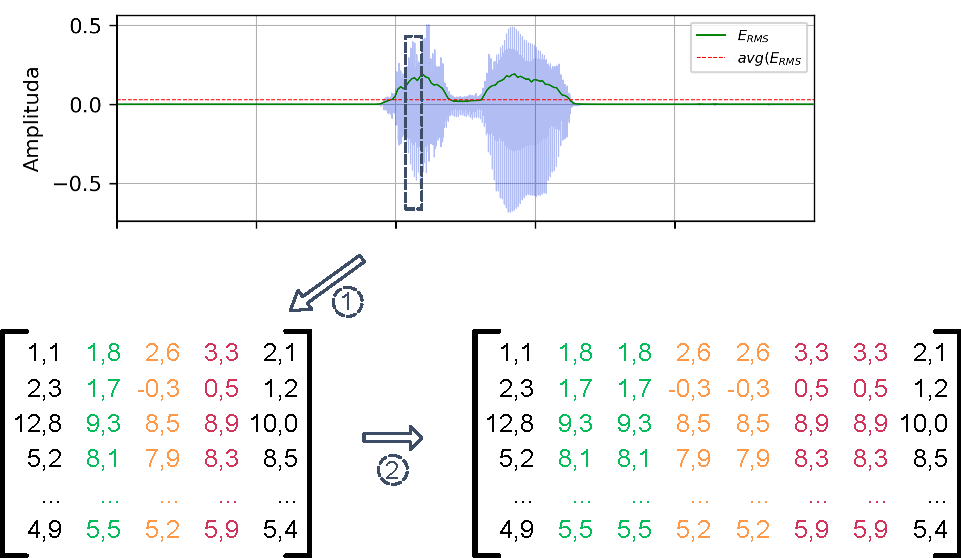
\includegraphics[width=0.9\textwidth]{./ch5-construction/img/augmentation_features.pdf}
%   \caption{Princip protažení na příznacích.}
%   \label{fig:realisation:augmentation:features}
% \end{figure}

\subsubsection{Dosažené výsledky}

% Prvním bodem výše zmíněného algoritmu bylo získat standardní model, který by bylo vhodné použít  k~zarovnání dat.
% Jako vhodné se jevilo použít již natrénovaný model z~experimentů popsaných v~části \ref{chap:realisation:corpus:elimination}.
% Tento model dosáhl s~fonémovým zerogramovým LM přesnosti rozpoznávání $84,66~\%$.
% S jeho pomocí bylo získáno zarovnání trénovací i testovací sady.

Pro prvotní ověřovací experiment bylo zvoleno $2\mathrm{x}$ protažení fonému $/s/$, tedy všechny vektory odpovídající $/s/$ byly zduplikovány.
% Následně byl standardním způsobem natrénován HMM-DNN model.
Otestování bylo jako v~předchozích případech realizováno na testovací sadě s~fonémovým zerogramovým jazykovým modelem, aby byl minimalizován vliv LM.
Tento nový model dosáhl přesnosti rozpoznávání $85,11~\%$.
% , což lze označit jako malé zlepšení oproti baseline HMM-DNN modelu.

Další experiment byl realizován na protažených fonémech $/k/$, $/p/$, $/s/$, $/t/$ a $/v/$, které reprezentují většinu neznělých zájmových fonémů.
Zarovnání bylo identické jako u předchozího experimentu, stejně tak bylo uvažováno jejich $2\mathrm{x}$ protažení, tzn. že všechny vektory inkriminovaných fonémů byly zduplikovány.
Znovu byl natrénován HMM-DNN model se stejnými parametry a násedně byl otestován s~fonémovým zerogramovým jazykovým modelem.
Přesnost rozpoznávání na testovací sadě dosáhla hodnoty $87,50~\%$, což lze považovat za významné zlepšení.

V další fázi bylo potřeba ověřit, zda jiné hodnoty násobku protažení nemohou poskytnout lepší výsledek.
Experiment byl zopakován pro $3\mathrm{x}$, $4\mathrm{x}$ a $5\mathrm{x}$ jejich původní délky.
Protaženy byly fonémy $/k/$, $/p/$, $/s/$, $/t/$ a $/v/$.
Proces natrénování a otestování modelu korespondoval s~předchozími experimenty.
Dosažené výsledky byly zaznamenány do tab. \ref{tab:realisation:augmentation:influence}.
Pro úplnost byla tabulka doplněna o baseline model neobsahuhjící protažení a model s~$2\mathrm{x}$ protažením.
Z uvedených výsledků je patrný jasný trend, větší než $2\mathrm{x}$ protažení vede ke zhoršení přesnosti rozpoznávání.
Optimální hodnota protažení tak teoreticky leží někde mezi jednonásobkem a trojnásobkem původní délky.
Bohužel uvedeným postupem nelze přesně určit hodnotu míry protažení.

\begin{table}[htpb]
  \centering
  \def\arraystretch{1.5}
  \pgfplotstabletypeset[
    col sep=semicolon,
    string type,
    columns/extension/.style={
      column name={},
      column type={l},
      string replace={accp}{$Acc_{p}\ [\%]$}
    },
    columns/1x/.style={column name=$1\mathrm{x}$, column type={r}},
    columns/2x/.style={column name=$2\mathrm{x}$, column type={r}},
    columns/3x/.style={column name=$3\mathrm{x}$, column type={r}},
    columns/4x/.style={column name=$4\mathrm{x}$, column type={r}},
    columns/5x/.style={column name=$5\mathrm{x}$, column type={r}},
    every head row/.style={
      after row={
        % \cmidrule{2-10}
        \midrule
      },
      before row={\toprule & \multicolumn{5}{c}{Míra protažení} \\}
    },
    every last row/.style={after row={\bottomrule}},
  ]{./parts/ch6-realisation/tabs/0301-features.csv}
  \caption{Vliv míry protažení na přesnost modelu.}
  \label{tab:realisation:augmentation:influence}
\end{table}

% Zhoršení přesnosti u vyšších hodnot míry protažení dozajista souvisí s~faktem, že výsledná augmentovaná data neodpovídají realitě.
% Čím vícekrát je vektor zkopírován, tím více je vnášena chyba způsobená ignorováním dynamické povahy signálu.
% Nicméně jako proof-of-concept myšlenky posloužil tento experiment velmi dobře.

\subsection{Protažení na zvuku}
\label{chap:realisation:augmentation:audio}

Protažení na příznacích vedlo sice  k~významnému zlepšení přesnosti rozpoznávání, ale tento přístup není bohužel reálně použitelný. Vhodnou alternativou může být model pracující s~fonémy protaženými přímo v~audio signálu.
Taková data budou teoreticky více odpovídat reálným datům získaným od řečníka.
Stejně jako v~předchozím případě je  k~protažení potřeba zarovnání.
To s~určitou mírou přesnosti určuje počáteční a koncové hranice jednotlivých fonémů.
S ohledem na stanovené hranice je možné určitý úsek protáhnout například pomocí

\begin{itemize}
  \item převzorkování signálu,
  \item TD-PSOLA algoritmu,
  \item fázového vokodéru.
\end{itemize}

\noindent Asi nejjednodušší metodou je převzorkování dat, pro jehož realizaci stačí načíst všechny vzorky odpovídající vybranému fonému a změnit jejich vzorkovací frekvenci.
Pokud je cílem tento úsek protáhnout, je nová vzorkovací frekvence menší než originální.
Hlavním problémem této metody je tonální posun\footnote{Mění se fundamentální frekvence $F_0$. Pokud dojde ke zrychlení, frekvence se zvýší. Při zpomalení naopak sníží.}.
% Přestože protahovaný úsek tvoří jen malou část z celkové délky nahrávky, cílem je vygenerovat takové protaženín nahrávky, které co nejvíce odpovídá realitě.
% Proto není protažení pomocí převzorkování nejvhodnější metodou.

Zbylé dva uvažované přístupy využívají sofistikovanější úpravy signálu v~časové oblasti.
Obě metody využívají \textit{analýzu} signálu, pro jeho následné \textit{zpracování}, které je zakončené \textit{syntézou}.
% Metody z rodiny PSOLA pracují s~hlasivkovými pulsy, které jsou nejprve v~analytické části nalezeny\footnote{Výsledkem analýzy jsou periodicky se opakující značky, angl. pitch marks. Úpravou jejich parametrů dochází ke změnám parametrů řeči.}, aby pak v~části zpracování došlo  k~jejich transformaci na základě požadavků na výslednou řeč.
% V posledním kroku dochází k~syntéze signálu na základě upravených analytických krátkodobých signálů (hlasivkových pulsů), podrobněji v~\cite{Psutka2006}.

% Fázový vokodér pracuje na podobném principu, s~tím rozdílem, že v~analytické části dochází  k~převodu signálu do frekvenční oblasti.
% Ve fázi zpracování je signál upraven tak, aby mohl být ve fázi syntézy opět převeden do časové oblasti.

Pomocí těchto dvou zmíněných metod je možné upravit nejen délku, ale i  fundamentální frekvenci $F_0$ signálu.
% Negativně se může úprava projevit např. vznikem artefaktů, které u TD-PSOLA vznikají v~důsledku nespojitosti mezi sousedními úseky řeči; u fázového vokodéru mohou vznikat artefakty např. vlivem fázového posunu.
% Obě metody však poskytují velmi dobré výsledky protažení na jednotlivých fonémech.
% Dosažené protažení je téměř identické.
% Přestože interně vyvinutý nástroj umožňuje k~ovlivnění délky řeči (a priori používaný pro účely řešení úlohy syntézy řeči) využít obě výše zmíněné metody, tak pro účely této práce byli protažení modelováno metodou TD-PSOLA.
% Ukázka původního a protaženého slova \uv{kosa} je na obr. \ref{fig:realisation:augmentation:compare}.
% Protahován byl foném $/s/$, který je v~signálu reprezentovaný šumem mezi dvěma výraznými částmi signálu.
% Inkriminovaný foném byl protažen na dvojnásobek.
% Na obr. \ref{fig:realisation:augmentation:compare:augmented} je pak zřetelně vidět protažení úseku odpovídající $/s/$.
% V signálu a ve spektru není vidět žádný významný artefakt.

% \begin{figure}[htpb]
%   \centering
%   \begin{subfigure}[b]{0.42\textwidth}
%     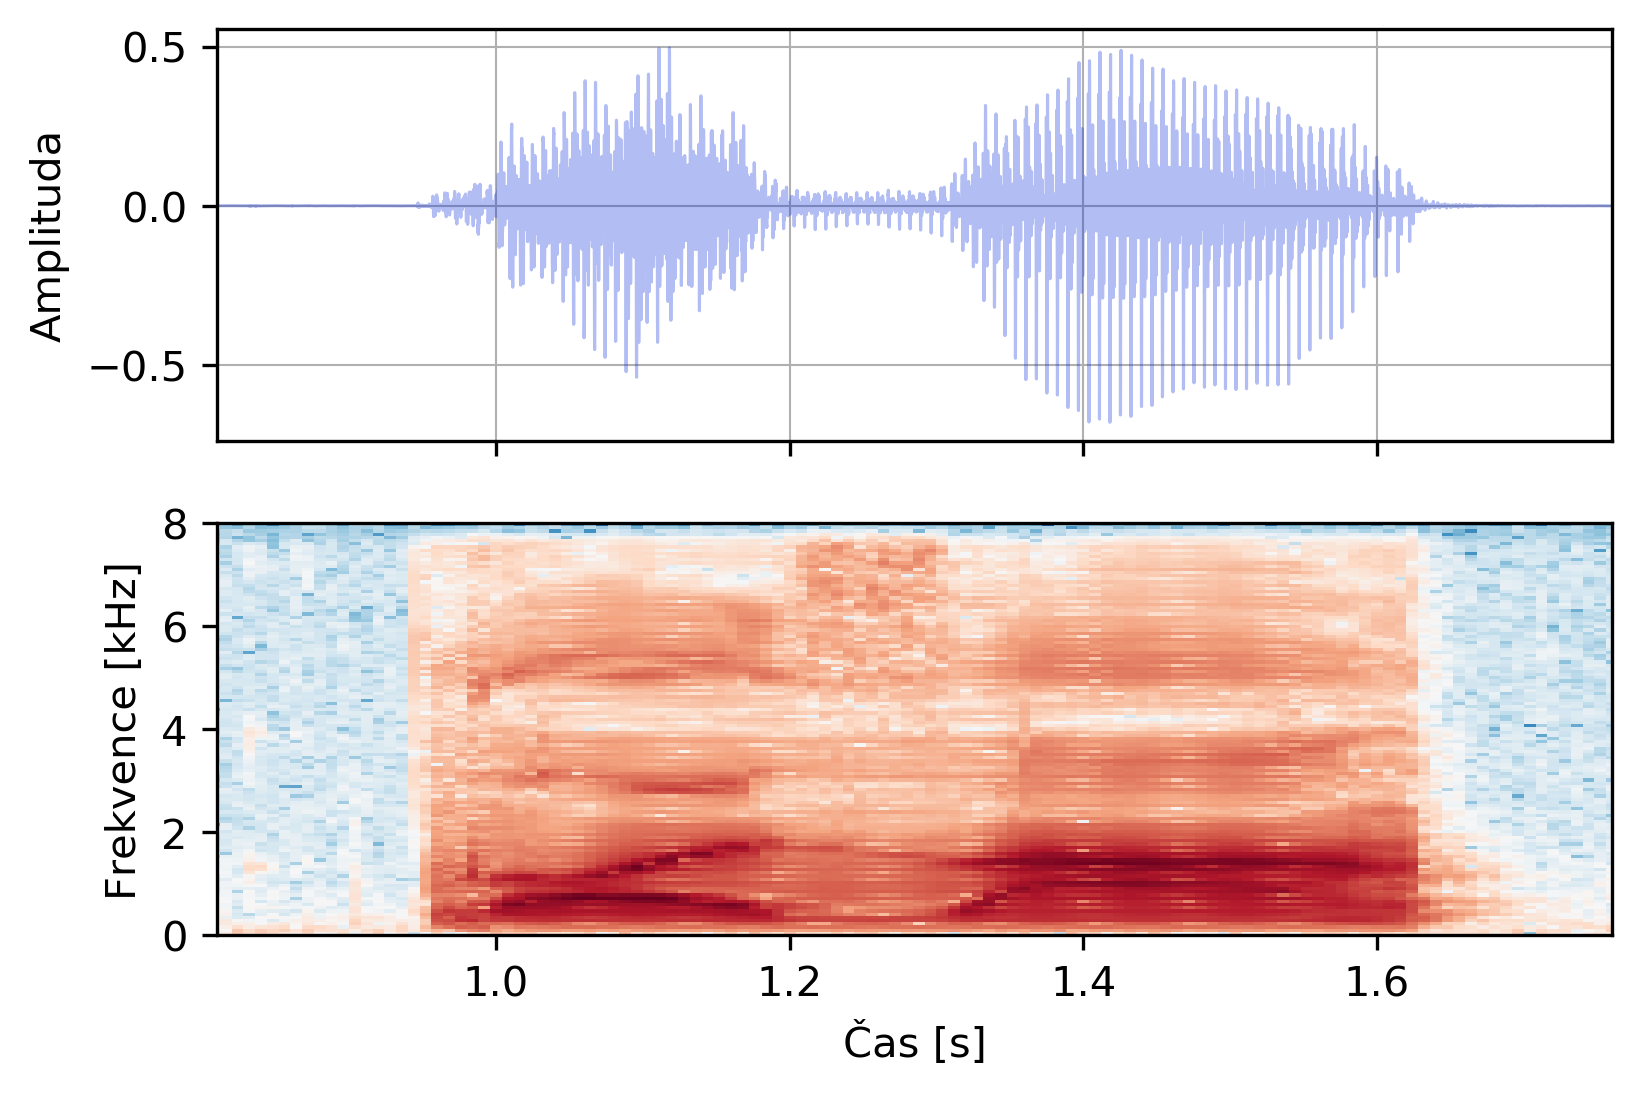
\includegraphics[width=\textwidth]{./ch6-realisation/img/energy_spec_word-kosa.png}
%     \caption{Originální}
%     \label{fig:realisation:augmentation:compare:original}
%   \end{subfigure}
%   %
%   \begin{subfigure}[b]{0.42\textwidth}
%     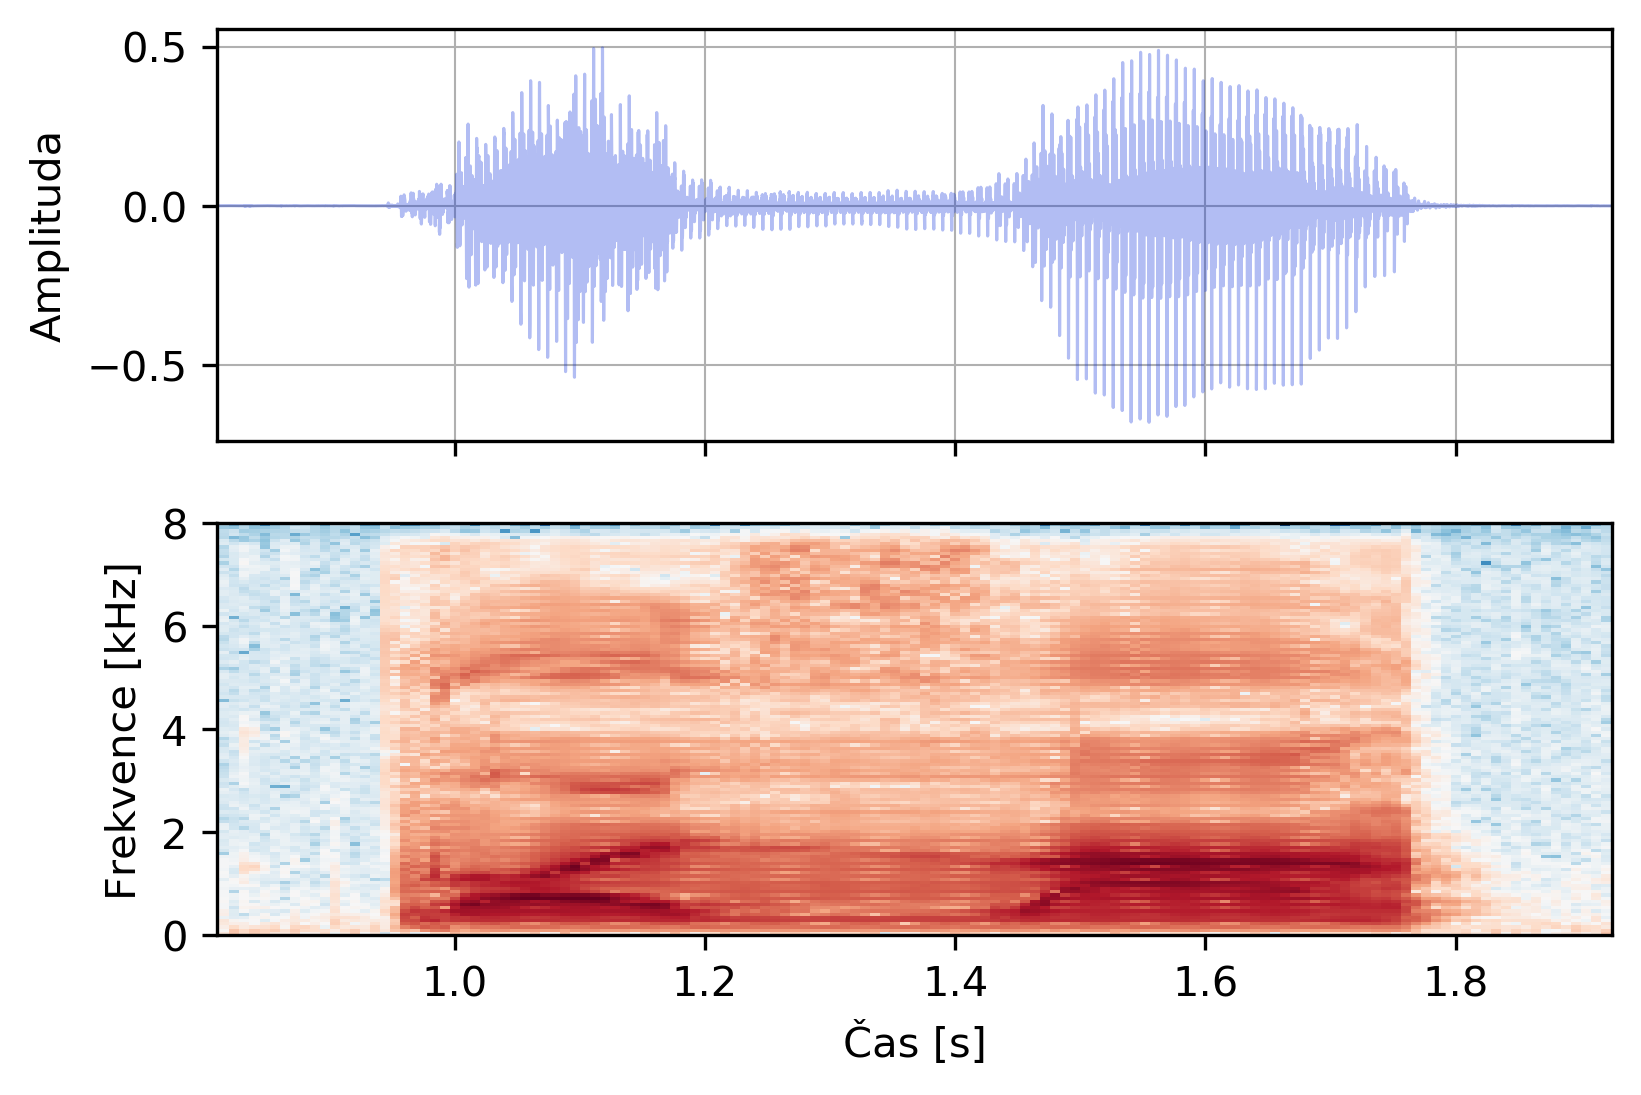
\includegraphics[width=\textwidth]{./ch6-realisation/img/energy_spec_word-kosa_real.png}
%     \caption{Protažené}
%     \label{fig:realisation:augmentation:compare:augmented}
%   \end{subfigure}
%   \caption{Amplituda a spektrogram původního (protaženého) slova \uv{kosa}.}
%   \label{fig:realisation:augmentation:compare}
% \end{figure}

\subsubsection{Dosažené výsledky s~DNN}

K ověření schopností modelu pracovat s~uměle protaženými daty byl použit stejný HMM-DNN model jako v~předchozích případech.
V datech jsou protaženy všechny výskyty fonémů $/k/$, $/p/$, $/s/$, $/t/$ a $/v/$. Uvažováno je protažení $1,25\mathrm{x}$, $1,50\mathrm{x}$, $1,75\mathrm{x}$ a $2,00\mathrm{x}$. Jazykový model je stejně jako v~případě protažení na příznacích fonémový zerogramový.
Dosažené výsledky jsou shrnuty v~tab. \ref{tab:realisation:augmentation:influence:dnn}.
Nejlepšího výsledku dosáhl \textit{baseline} model s~hodnotou $84,66~\%$.
S libovolným protažením dochází  k~poklesu přesnosti.

\begin{table}[htpb]
  \centering
  \def\arraystretch{1.5}
  \pgfplotstabletypeset[
    col sep=semicolon,
    string type,
    columns/extension/.style={
      column name={},
      column type={l},
      string replace={accp}{$Acc_{p}\ [\%]$}
    },
    columns/100/.style={column name={$1,00\mathrm{x}$}, column type={r}},
    columns/125/.style={column name={$1,25\mathrm{x}$}, column type={r}},
    columns/150/.style={column name={$1,50\mathrm{x}$}, column type={r}},
    columns/175/.style={column name={$1,75\mathrm{x}$}, column type={r}},
    columns/200/.style={column name={$2,00\mathrm{x}$}, column type={r}},
    every head row/.style={
      after row={
        % \cmidrule{2-6}
        \midrule
      },
      before row={\toprule & \multicolumn{5}{c}{Míra protažení} \\}
    },
    every last row/.style={after row={\bottomrule}},
  ]{./parts/ch6-realisation/tabs/0302-audio_1.csv}
  \caption{Vliv míry protažení fonému na přesnost DNN modelu.}
  \label{tab:realisation:augmentation:influence:dnn}
\end{table}

\subsubsection{Upravené zarovnání a time delay neural network}

Při analýze výsledků se ukázalo, že zarovnání v~mnoha případech není zrovna nejpřesnější, a to zvláště u inkriminovaných neznělých fonémů.
% Na obr. \ref{fig:realisation:augmentation:alignemnt:wrong} je ukázáno získané zarovnání slova \uv{kosa} společně s~vyznačenými hranicemi v~audiu signálu a spektru.
% Z obr. \ref{fig:realisation:augmentation:alignemnt:wrong:audio} je zřejmé, že počáteční hranice fonému $/s/$ zasahuje do předchozího fonému $/o/$.
% Tím pádem dochází  k~protažení nevhodné části signálu a model se tak učí na špatných datech.
% Pokud by všechny fonémy $/s/$ následovaly po fonému $/o/$, tak by se nejednalo o závažný problém, ale toto samozřejmě neplatí.
% V~době, kdy byly prováděny experimenty s~protažením konkrétních fonémů, se začaly stále více prosazovat time-delay neural networks (TDNN).
% Přestože patří do rodiny feed-forward sítí jako DNN, tak se oproti nim snaží vzít v~potaz i dynamickou složku řeči, podrobněji v~části \ref{chap:asr:acoustic:DNN}.

% \begin{figure}[htpb]
%   \centering
%   \begin{subfigure}[b]{0.26\textwidth}
%     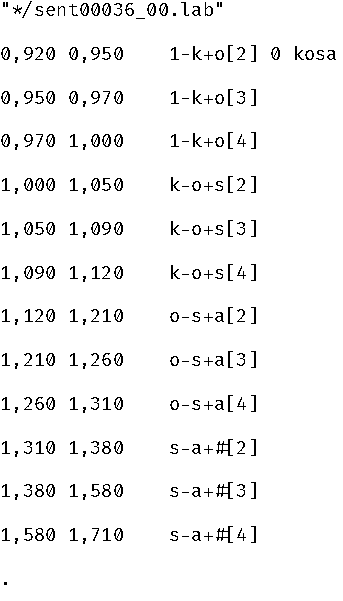
\includegraphics[width=\textwidth]{./ch6-realisation/img/alignment_text.pdf}
%     \caption{Zarovnání}
%     \label{fig:realisation:augmentation:alignemnt:wrong:text}
%   \end{subfigure}
%   %
%   \begin{subfigure}[b]{0.65\textwidth}
%     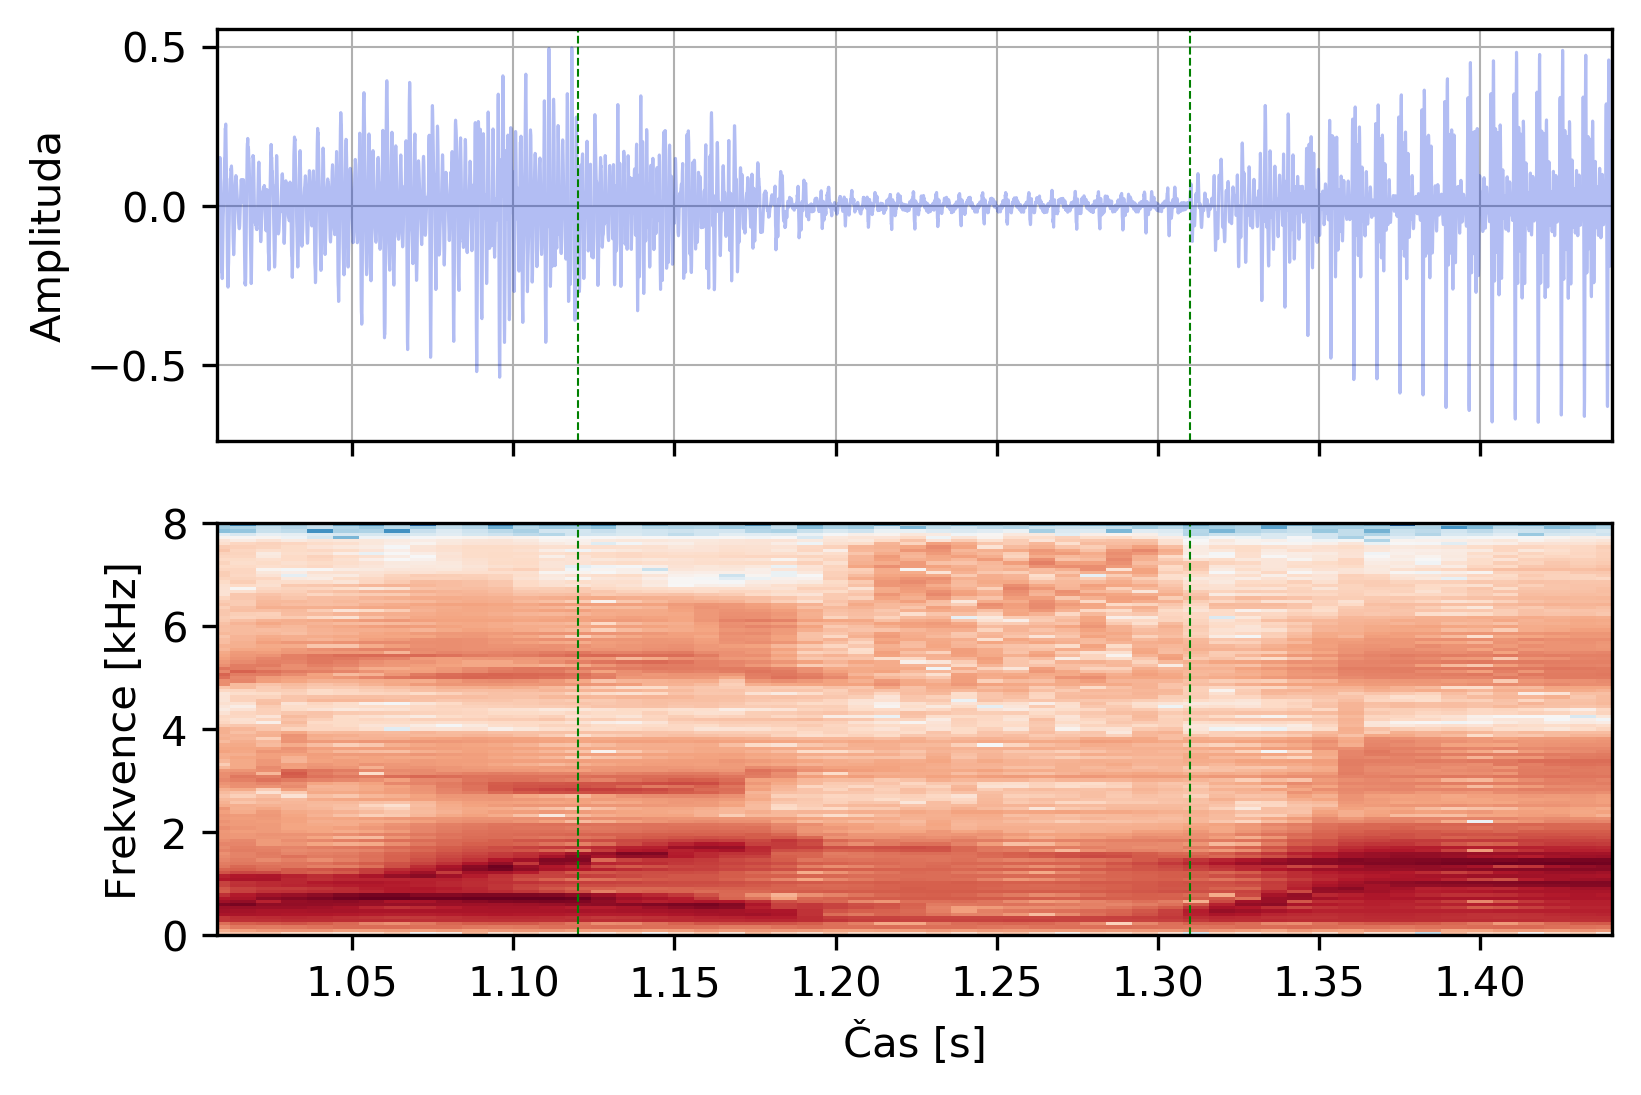
\includegraphics[width=\textwidth]{./ch6-realisation/img/energy_spec_word-segment.png}
%     \caption{V signálu}
%     \label{fig:realisation:augmentation:alignemnt:wrong:audio}
%   \end{subfigure}
%   \caption{Špatně zarovnaný foném $/s/$ ve slově \uv{kosa}.}
%   \label{fig:realisation:augmentation:alignemnt:wrong}
% \end{figure}

% Stejně jako u DNN modelu je na počátku trénování nutné mít  k~dispozici zarovnání.
% To ale nemusí být naprosto přesné, protože je vstupní vektor zpracováván jiným způsobem než u DNN.
% Díky FIR filtraci a více množinám vah je brán v~potaz i dynamický charakter řeči \cite{Peddinti2015}.
% Model založený na TDNN by tak měl generovat přesnější zarovnání, tedy zlepšit výsledky modelu pracujícího s~uměle protaženými daty.

% Jako startovní bod trénování je použito DNN zarovnání z předchozího experimentu. Topologie sítě vychází z hodnot prezentovaných v~\cite{Peddinti2015}, tedy síť má $4$ skryté vrstvy. Každá vrstva má 650 neuronů. První vrstva pracuje s~kontextem $t-2$ a $t+2$, druhá vrstva s~$t-1$ a $t+2$, třetí vrstva s~$t-3$ a $t+4$ a čtvrtá s~$t-7$ a $t+2$. Výpočet výstupu pak bere v~potaz kontext $t-13$ a $t+9$ mikrosegmentů, viz \cite{Peddinti2015}.

% Na obr. \ref{fig:realisation:augmentation:alignemnt:correct} je zobrazeno získané zarovnání slova \uv{kosa} TDNN modelem.
% Z vyznačených hranic fonému $/s/$ (obr. \ref{fig:realisation:augmentation:alignemnt:correct:audio}) je patrné v~podstatě přesné zarovnání.
% Přesnost TDNN modelu s~fonémovým zerogramovým jazykovým modelem dosáhla hodnoty $Acc_{p}= 85,41~\%$.

% \begin{figure}[htpb]
%   \centering
%   \begin{subfigure}[b]{0.26\textwidth}
%     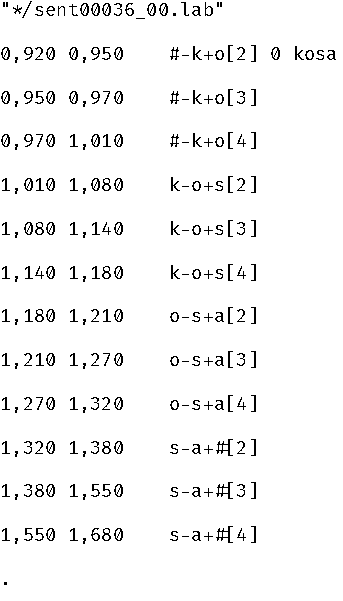
\includegraphics[width=\textwidth]{./ch6-realisation/img/alignment_text-2.pdf}
%     \caption{Zarovnání}
%     \label{fig:realisation:augmentation:alignemnt:correct:text}
%   \end{subfigure}
%   %
%   \begin{subfigure}[b]{0.65\textwidth}
%     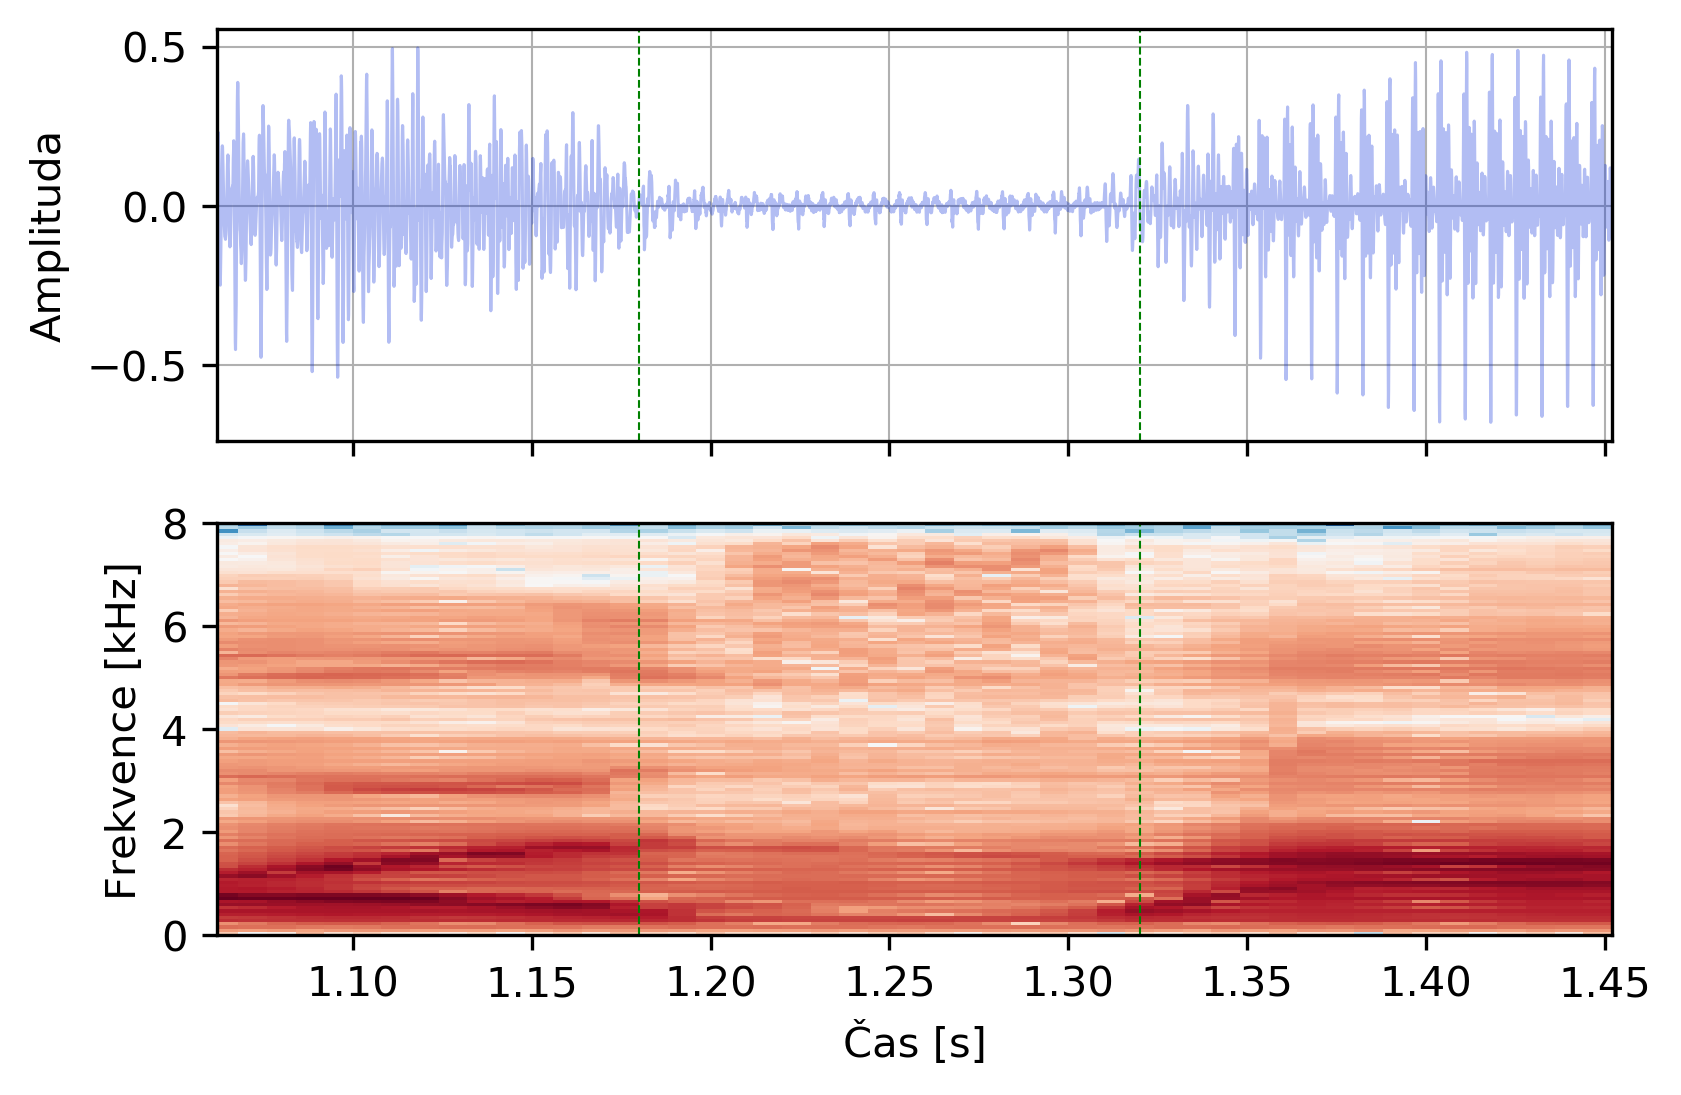
\includegraphics[width=\textwidth]{./ch6-realisation/img/energy_spec_word-segment-2.png}
%     \caption{V signálu}
%     \label{fig:realisation:augmentation:alignemnt:correct:audio}
%   \end{subfigure}
%   \caption{Správně zarovnaný foném $/s/$ ve slově \uv{kosa}.}
%   \label{fig:realisation:augmentation:alignemnt:correct}
% \end{figure}

S přesnějším zarovnáním je možné přistoupit  k~protažení fonémů $/k/$, $/p/$, $/s/$, $/t/$, $/v/$ a vytvoření nového modelu pracujícího s~těmito daty.
Jako další model je tedy použita TDNN síť.
K otestování modelu je využit standardní fonémový zerogramový jazykový model.
Uvažováno je protažení od $1,25\mathrm{x}$ do $3,00\mathrm{x}$ s~krokem $0,25$. Výsledky experimentu jsou uvedeny v~tab. \ref{tab:realisation:augmentation:influence:tdnn}.
Oproti hodnotám rozpoznávání přesnosti v~tab. \ref{tab:realisation:augmentation:influence:dnn} je vidět výrazné zlepšení přesnosti oproti baselinu modelu ($Acc_{p} = 85,41~\%$).
Nejvyšší přesnosti $87,90~\%$ dosáhl model pracující s~$2,5\mathrm{x}$ protaženými daty, navíc modely pracující s~protažením od $1,75\mathrm{x}$ do $2,75\mathrm{x}$ dosahují velmi blízkých hodnot přesnosti rozpoznávání.
To poskytuje relativně široký pracovní interval pro případné skutečné protažení dat řečníkem.

\begin{table}[htpb]
  \centering
  \def\arraystretch{1.5}
  \pgfplotstabletypeset[
    col sep=semicolon,
    string type,
    columns/extension/.style={
      column name={},
      column type={l},
      string replace={accp}{$Acc_{p}\ [\%]$}
    },
    columns/100/.style={column name={$1,00\mathrm{x}$}, column type={r}},
    columns/150/.style={column name={$1,50\mathrm{x}$}, column type={r}},
    columns/125/.style={column name={$1,25\mathrm{x}$}, column type={r}},
    columns/175/.style={column name={$1,75\mathrm{x}$}, column type={r}},
    columns/200/.style={column name={$2,00\mathrm{x}$}, column type={r}},
    columns/225/.style={column name={$2,25\mathrm{x}$}, column type={r}},
    columns/250/.style={column name={$2,50\mathrm{x}$}, column type={r}},
    columns/275/.style={column name={$2,75\mathrm{x}$}, column type={r}},
    columns/300/.style={column name={$3,00\mathrm{x}$}, column type={r}},
    every head row/.style={
      after row={
        % \cmidrule{2-10}
        \midrule
      },
      before row={\toprule & \multicolumn{9}{c}{Míra protažení} \\}
    },
    every last row/.style={after row={\bottomrule}},
  ]{./parts/ch6-realisation/tabs/0303-audio_2.csv}
  \caption{Vliv míry protažení fonému na přesnost TDNN modelu.}
  \label{tab:realisation:augmentation:influence:tdnn}
\end{table}

Podstatnou otázkou je robustnost modelu.
S ohledem na hodnoty přesnosti rozpoznávání uvedené v~tab. \ref{tab:realisation:augmentation:influence:tdnn:robust} se dá říci, že duration model je v~rámci možností robustní v~poměrně širokém rozsahu protažení.
Očekávaným výsledkem je nejnižší hodnota přesnosti rozpoznávání pro neprotažená data (konkrétně $78,61~\%$).
Většina chyb v~rozpoznávání nastala v~důsledku neznalosti inkriminovaných neprotažených fonémů.
Tento výsledek je předpokladem pro funkci trenažéru prezentovaného v~části \ref{chap:realisation:trainer}.

\begin{table}[htpb]
  \centering
  \def\arraystretch{1.5}
  \pgfplotstabletypeset[
    col sep=semicolon,
    string type,
    columns/extension/.style={
      column name={},
      column type={l},
      string replace={accp}{$Acc_{p}\ [\%]$}
    },
    columns/100/.style={column name={$1,00\mathrm{x}$}, column type={r}},
    columns/150/.style={column name={$1,50\mathrm{x}$}, column type={r}},
    columns/125/.style={column name={$1,25\mathrm{x}$}, column type={r}},
    columns/175/.style={column name={$1,75\mathrm{x}$}, column type={r}},
    columns/200/.style={column name={$2,00\mathrm{x}$}, column type={r}},
    columns/225/.style={column name={$2,25\mathrm{x}$}, column type={r}},
    columns/250/.style={column name={$2,50\mathrm{x}$}, column type={r}},
    columns/275/.style={column name={$2,75\mathrm{x}$}, column type={r}},
    columns/300/.style={column name={$3,00\mathrm{x}$}, column type={r}},
    every head row/.style={
      after row={
        % \cmidrule{2-10}
        \midrule
      },
      before row={\toprule & \multicolumn{9}{c}{Míra protažení} \\}
    },
    every last row/.style={after row={\bottomrule}},
  ]{./parts/ch6-realisation/tabs/0305-robust.csv}
  \caption{Robustnost nejlepšího TDNN modelu ($2,5\mathrm{x}$) na míru protažení.}
  \label{tab:realisation:augmentation:influence:tdnn:robust}
\end{table}

Experimenty s~uměle protaženými daty potvrdily správnost uvažované hypotézy.
Protažením jednoho z párových fonémů dojde  k~dostatečnému odlišení velmi podobných zvukových reprezentací.
Tím dojde  k~natrénování odlišných modelů fonémů v~HMM.
Model pracující s~fonémy protaženými přímo ve zvuku nakonec dosáhl lepších výsledků než model s~uměle protaženými daty na příznacích.
% Svůj podíl na tom má i použití TDNN modelu.
% Model pracující s~duplikovanými příznaky naznačoval, že optimální hodnota protažení bude v~intervalu jedno až trojnásobku, což druhý typ modelu potvrdil.

\subsection{Aktualizace výsledků porovnání}
\label{chap:realisation:augmentation:comparison}

V části \ref{chap:realisation:listening} byla prezentováno srovnání schopností člověka a stroje.
Posloužily k~tomu dva poslechové testy a celkem $3$ ASR experimenty \uv{one-mil}, \uv{reduced} a \uv{bigrams}.
S využitím nového modelu je možné aktualizovat hypotetické výsledky stroje.
Hypotetické z toho důvodu, že použitá data jsou uměle protažena.
% Nicméně to nebrání provedení tohoto experimentu.
% Získané hodnoty mohou být brány jako jakási teoretická maxima ASR systému.
% Uměle upravená data budou relativně přesně a konzistentně protažena, u reálných dat toto nelze a priori očekávat.

K aktualizaci výsledků byl použit
%nejlepší
model z části \ref{chap:realisation:augmentation:audio}, tedy ten s~$2,5\mathrm{x}$ protaženými daty.
% Parametry experimentů byly totožné s~těmi v~části \ref{chap:realisation:listening}.
% V případě experimentu \uv{one-mil} byl použit zerogramový jazykový model s~1 milionem slov, experiment \uv{reduced} pak pouze zerogramový LM se slovy obsaženými v~poslechovém testu ($N = 320$).
% Speciální LM, obsahující 4 kombinace slov, byl vygenerován pro každou položku \uv{bigrams} experimentu.

% Dosažené výsledky byly zaznamenány do tab. \ref{tab:realisation:augmentation:comparison}.
% Ve všech třech případech došlo  k~významnému zlepšení.
% U experimentu \uv{one-mil} to je o~$23~\%$ absolutně, u~\uv{reduced} experimentu pak o~$24~\%$.
% K nejmarkantnějšímu zlepšení došlo u experimentu \uv{bigrams}, dokonce o~$44~\%$.
% Výsledky člověka se nezměnily, protože realizace poslechového testu je zdlouhavý proces a je obtížné získat dostatečný počet respondentů.
% Nicméně se dá očekávat, že i člověk by dosáhl zlepšení.
% Pokud by měl informaci o fonémech, které jsou protaženy.
% V opačném případě by ke zlepšení nutně nemuselo dojít, protože kromě protažení nebyl zvuk nijak pozměněn.

% Velmi zajímavé je porovnání zvýšení přesnosti rozpoznávání TDNN modelu s~fonémovým zerogramovým LM ($2,49~\%$ absolutně mezi baseline a $2,5\mathrm{x}$ modelem, viz tab. \ref{tab:realisation:augmentation:influence:tdnn}) a dosaženými výsledky prezentovanými v~tab. \ref{tab:realisation:augmentation:comparison}.
% Oproti nim je zlepšení o~$2,49~\%$ absolutně poměrně zanedbatelné, přesto velmi významné zlepšení.
% Jasně to ukazuje ideu experimentů s~fonémovým zerogramovým jazykovým modelem.
% I drobné zlepšení u akustického modelu může vést  k~rapidnímu zlepšení sofistikovanějšího systému.

% \begin{table}[htpb]
%   \centering
%   \def\arraystretch{1.5}
%   \pgfplotstabletypeset[
%     col sep=semicolon,
%     string type,
%     columns/type/.style={column name=, column type={l}},
%     columns/onemil/.style={column name={one-mil}, column type={r}},
%     columns/reduced/.style={column name=reduced, column type={r}},
%     columns/bigrams/.style={column name=bigrams, column type={r}},
%     every head row/.style={
%       after row={
%         % \cmidrule(lr){1-1}
%         % \cmidrule(lr){2-4}
%         \midrule
%       },
%       before row={\toprule & \multicolumn{3}{c}{$Acc_{p}\ [\%]$} \\}
%     },
%     every last row/.style={
%       after row={\bottomrule},
%       before row={\midrule}
%     },
%   ]{./ch6-realisation/tabs/0304-comparison.csv}
%   \caption{Aktualizované porovnání dosažených výsledků člověka a stroje.}
%   \label{tab:realisation:augmentation:comparison}
% \end{table}

\subsection{Reálně protažená data}
\label{chap:realisation:augmentation:real}

% Získané výsledky s~uměle protaženými daty potvrdily hypotézu, že model pracující s~těmito daty může dosahovat lepších výsledků.
% Dalším krokem bylo získání reálně protažených dat.
% Nahrávání je relativně zdlouhavý proces,
% proto je nezbytné dobře vybrat správné promluvy.
% Problémem je navíc samotné protažení.
% Pokud by bylo cílem získat protažené celé slovo, lze řečníka instruovat, aby mluvil pomaleji.
% To ale cílem není.
% Výsledné promluvy mají mít protažené pouze určité fonémy, a to přibližně na dvojnásobek.
% Jako nejjednodušší, a svým způsobem i elegantní, se ukázal zápis se zdvojenými písmeny, která mají představovat protažený foném, např. \uv{kossa}.
% Řečník je obeznámen s~tím, že pokud slovo v~promluvě obsahuje tento dvojitý zápis, měl by se pokusit toto slovo patřičným způsobem protáhnout.
% Tento zápis navíc řečníka podvědomě \uv{nutí} vyslovit slovo jinak než v~případě normálního zápisu.

Nahrávání se zhostil stejný řečník jako v~1. a 2. etapě.
Tedy žena v~důchodovém věku, která používá EL v~běžném životě již více než 15 let.
Nahrávání se uskutečnilo v~průběhu 5 měsíců od července 2018 do listopadu 2018.
Texty určené k~nahrávání obsahovaly většinu izolovaných slov z poslechového testu a věty, které doposud neobsahuje řečový korpus složený z 1. a 2. etapy nahrávání.
Řečník byl instruován, aby slova, která obsahují zdvojená písmena (např. \uv{kossa}), adekvátně prodloužil.
% Nahrávání bylo realizováno za stejných podmínek jako v~2. etapě nahrávání (viz \ref{chap:realisation:corpus}).
% Nahrávání byl vždy přítomen operátor, který kontroloval, zda se řečník nevědomky nedopustil chyby či přeřeknutí.
% Stejně jako v~předchozí etapě obsahuje každá nahrávka minimálně $0,5\ s$ pauzu na začátku a konci.
% Celkem se takto v~rámci 3. etapy nahrávání podařilo získat dohromady $998$ promluv obsahující věty a slova (protažená i neprotažená), kterých je $267$.
Celkový čas promluv v~3. etapě dosáhl $2$ hodin a $28$ minut.

% Na obr. \ref{fig:realisation:real:compare} je zobrazena amplituda a spektrogram slova \uv{kose} protaženého řečníkem (\ref{fig:realisation:real:compare:real}) a 2x uměle (\ref{fig:realisation:real:compare:augmented}).
% Hlavním viditelným rozdílem je slabší zastoupení frekvencí kolem $2\ kHz$ ve spektrogramu mezi časem $3,2\ s$ a $3,4\ s$.
% Ač to tak na první pohled nevypadá, tak obě protažení mají téměř identickou délku $0,258\ s$ (reálné) vs. $0,261\ s$ (umělé).
% Vizuální rozdíl je způsoben vyšší celkovou délkou reálně protaženého slova.
% Foném $/s/$ je zástupcem neznělých fonémů, zdrojem zvuku je tedy a priori šum a nikoli periodický signál produkovaný hlasivkami, tím pádem je velikost amplitudy taktéž velmi podobná.
% Další viditelný rozdíl v~místě protažení fonému $/s/$ je způsoben vyšší maximální amplitudou u uměle protažené nahrávky (\ref{fig:realisation:real:compare:augmented}), která byla pořízena v~průběhu 2. etapy nahrávání.

% \begin{figure}[htpb]
%   \centering
%   \begin{subfigure}[b]{0.42\textwidth}
%     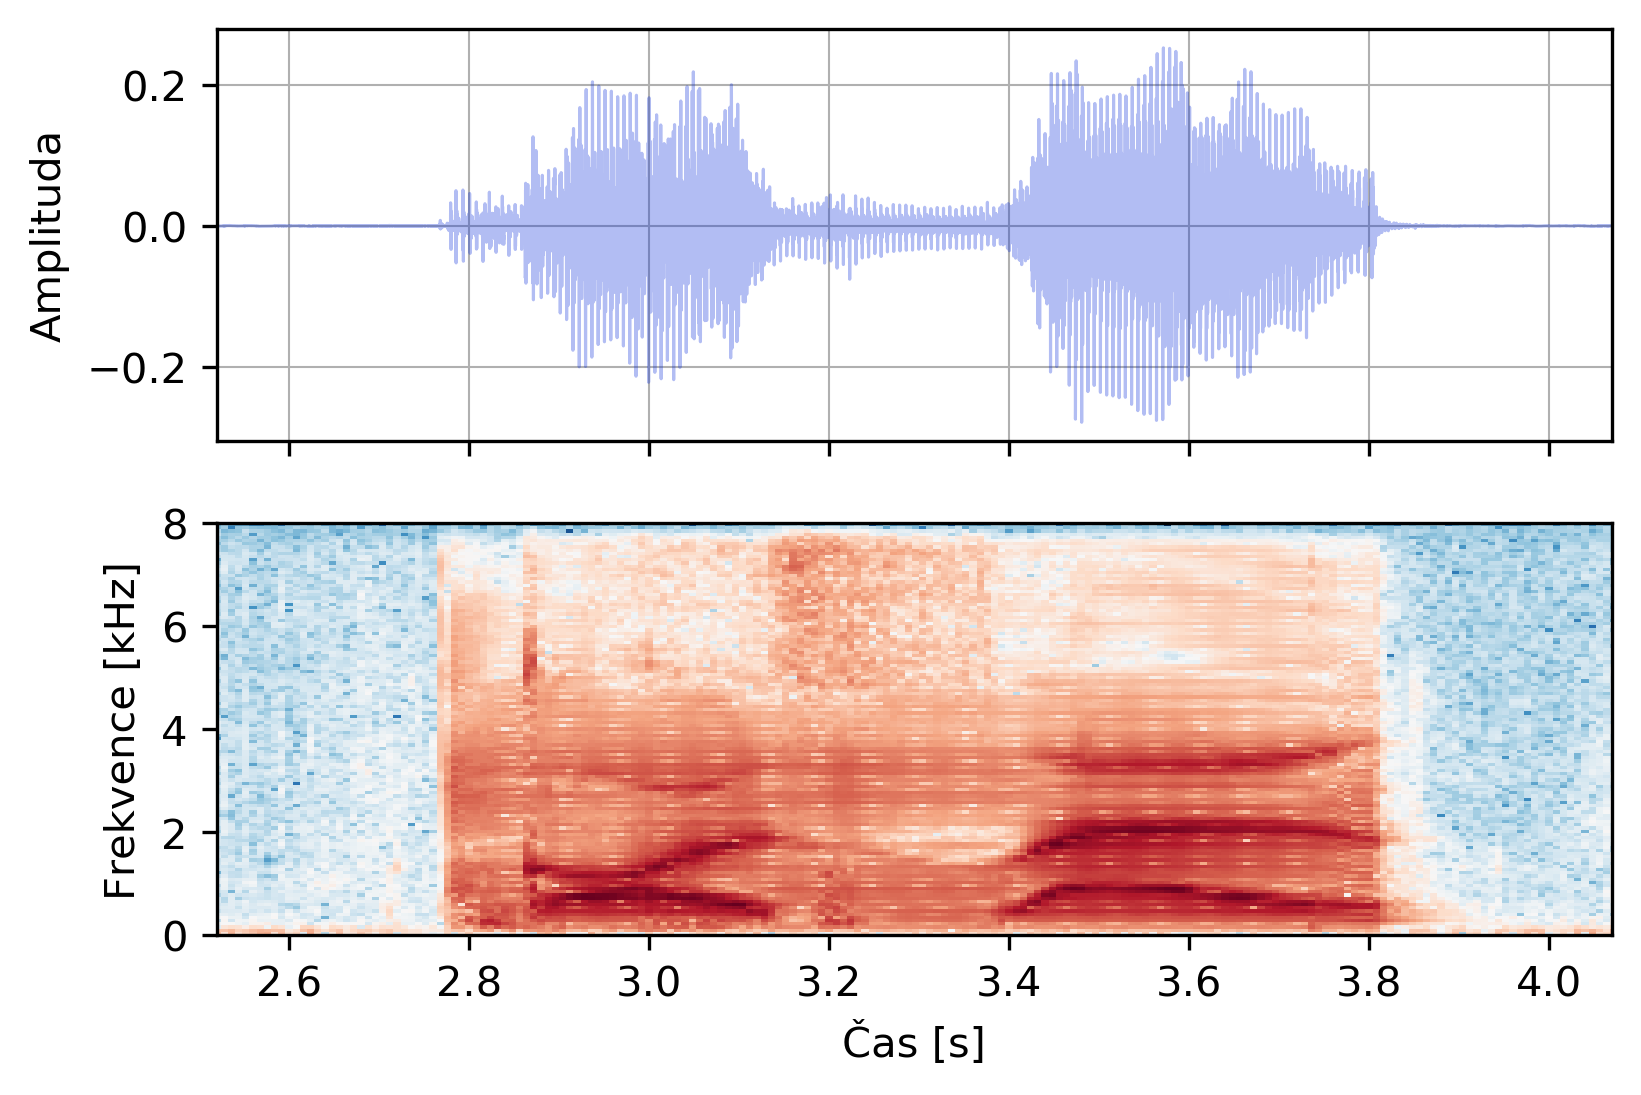
\includegraphics[width=\textwidth]{./ch6-realisation/img/energy_spec_word-kose_real.png}
%     \caption{Protažené řečníkem}
%     \label{fig:realisation:real:compare:real}
%   \end{subfigure}
%   %
%   \begin{subfigure}[b]{0.42\textwidth}
%     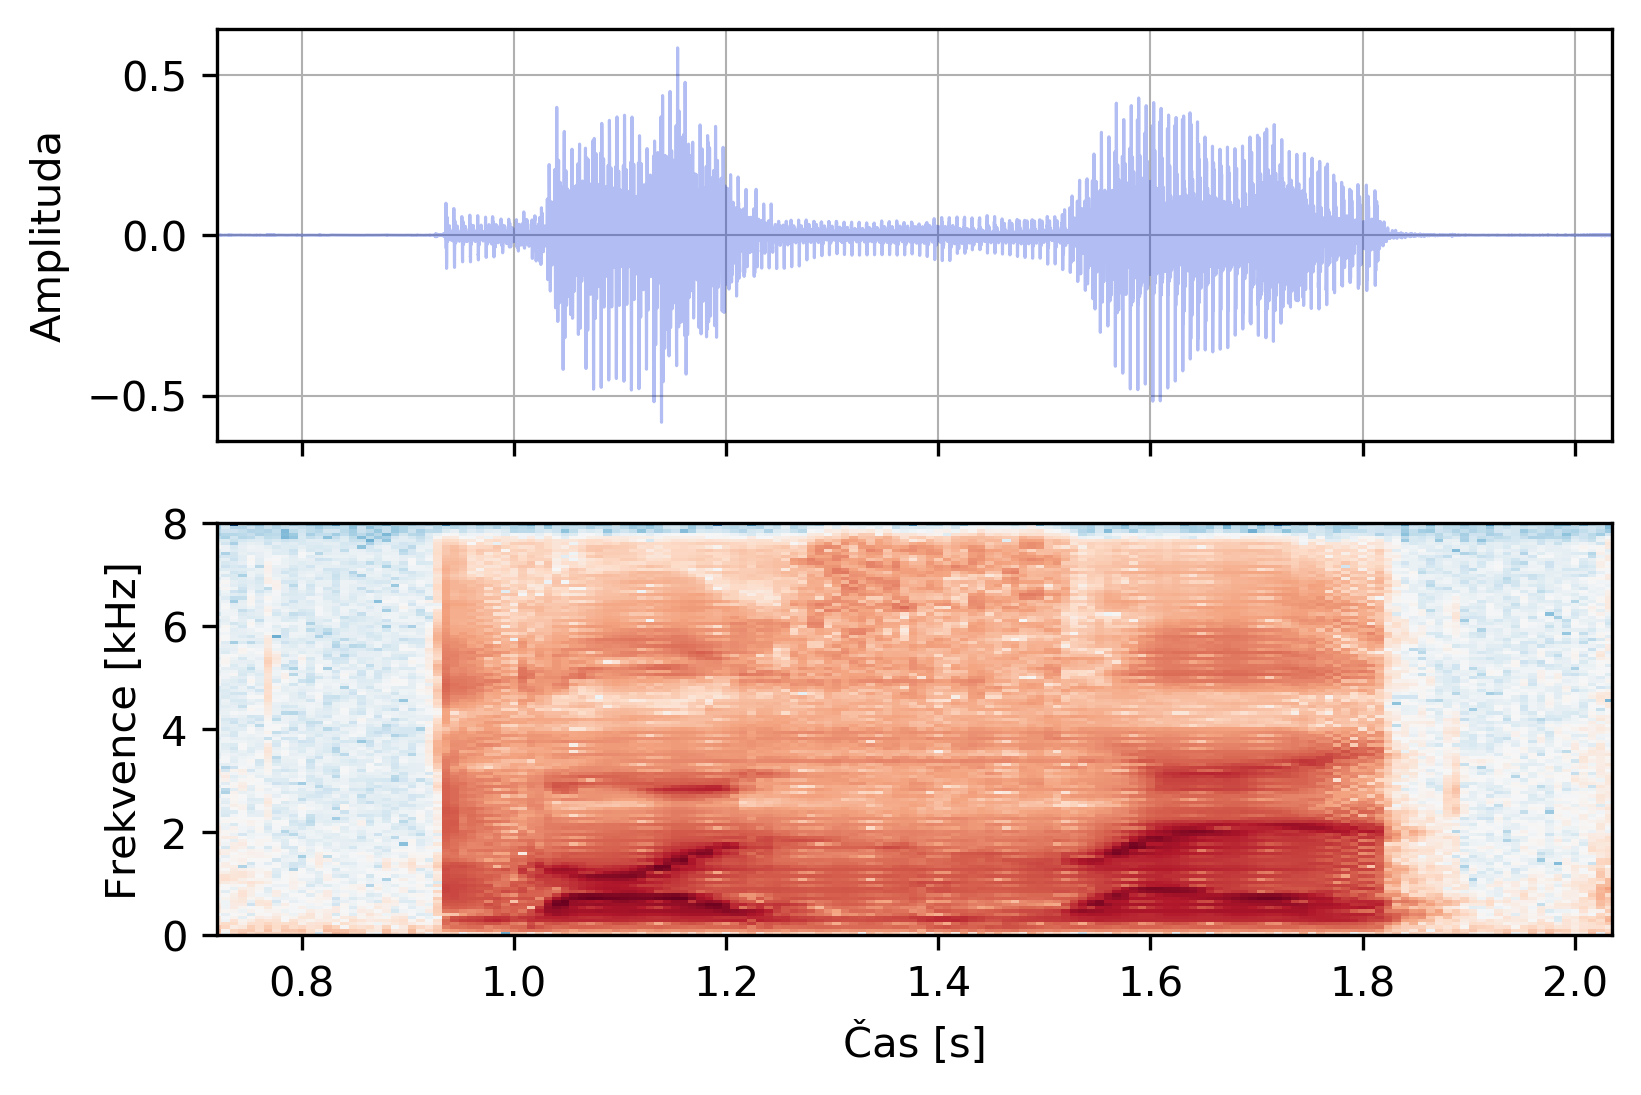
\includegraphics[width=\textwidth]{./ch6-realisation/img/energy_spec_word-kose_augmented.png}
%     \caption{Uměle protažené}
%     \label{fig:realisation:real:compare:augmented}
%   \end{subfigure}
%   \caption{Amplituda a spektrogram slova \uv{kose} protažené řečníkem/uměle.}
%   \label{fig:realisation:real:compare}
% \end{figure}

Hlubší analýza pořízených slov ve 3. etapě nahrávání ukázala, že proces umělého protažení produkuje svými charakteristikami velmi podobné nahrávky těm reálným.
Pro vytvoření modelu pouze z reálně protažených dat se však nepodařilo získat dostatečné množství dat.
Pokud jsou reálně protažená data opravdu velmi podobná uměle protaženým datům, tak by mělo být možné dosáhnout dobrých výsledků s~modelem, který je natrénovaný na uměle protažených datech, ale otestovaný těmi reálně protaženými.

% Porovnáním neprotažených nahrávek z 2. etapy a protažných nahrávek z 3. etapy se jako ideální jeví použití $2\mathrm{x}$ protaženého modelu z části \ref{chap:realisation:augmentation:audio} (viz tab. \ref{tab:realisation:augmentation:influence:tdnn}).
% Jedná se tedy o TDNN model, který je natrénován na datech obsahujících $2\mathrm{x}$ protažené fonémy $/k/$, $/p/$, $/s/$, $/t/$ a $/v/$.
% Na testovací sadě dosáhl přesnosti $Acc_{p} = 87,71~\%$.
% K otestování výkonu na reálně protažených datech jsou použity všechny věty a slova obsahující protažení zmíněných fonémů\footnote{Stejně jako u 1. a 2. etapy bylo i zde aplikováno CMN napočítané přes všechny nahrávky v~rámci etapy.}.
% S touto testovací sadou dosáhl zmíněný model s~fonémovým zerogramovým jazykovým modelem $Acc_{p} = 84,51~\%$.

% Dosažená přesnost je sice horší něž původní přesnost na uměle protažených datech, ale nedošlo  k~dramatickému propadu jako v~případě křížového testu mezi 1. a 2. etapou (viz tab. \ref{tab:realisation:verification:cmn:full}\footnote{V tabulce jsou prezentovány hodnoty odpovídající GMM modelu. Srovnání na první pohled není úplně korektní, nicméně validní, protože GMM model trénovaný na uměle protažených datech a otestovaný na reálně protažených datech dosáhl $Acc_{p} = 81,29~\%$, což je srovnatelná hodnota s~ostatními GMM modely.}).
% Dosažený výsledek tak potvrzuje podobnost uměle a reálně protažených dat.

V případě, že se k~trénovací sadě přidaly věty z 3. etapy, které neobsahují protažené fonémy, výsledná přesnost TDNN modelu s~fonémovým zerogramovým jazykovým modelem dosáhla hodnoty $Acc_{p} = 85,88~\%$.
To je lepší hodnota než v~případě baseline TDNN model ($Acc_{p} = 85,41~\%$, viz tab. \ref{tab:realisation:augmentation:influence:tdnn}).
Tyto experimenty podporují ideu trenažéru prezentovaného v~části \ref{chap:realisation:trainer}.

% !TEX root = ../thesis.tex
\section{Model akcentující protažení dat}
\label{chap:realisation:durationmodels}

Augmentace dat (viz část \ref{chap:realisation:augmentation}) ukázala, že ztracenou informaci EL řeči je částečné možné nahradit protažením inkriminovaných fonémů. Experimenty s reálně protaženými daty (viz část \ref{chap:realisation:augmentation:real}) navíc prokázaly schopnost člověla toto protažení realizovat. Dalším krokem je tedy úprava modelu tak, aby tuto změnu co možná nejvíce reflektoval.

Z principu fungování a nejpoužívanější topologie HMM modelu (viz \ref{chap:asr:acoustic:HMM}) je délka fonému modelována pomocí přechodových pravděpodobností. Ty zase vedou na funkce geometrické distribuce pravděpodobnosti \cite{Rabiner1989}. Bohužel skutečná podoba těchto distribucí odpovídá spíše gamma nebo logaritmicko-normálnímu rozdělení \cite{Alumae2014}.

Správné modelování délky může být realizováno úpravou přechodových hustotních funkcí v HMM nebo změnou topologie modelu. Druhou možností je vytvoření speciálního modelu pracujícího s délkou jednotlivých fonémů (duration model) a reskórováním výstupních N-best hypotéz či celé rozpoznávací mřížky.

Přestože se první uvažovaný způsob jeví jako vhodnější, tak všechny dosavadní publikované výsledky ukazují významné zvýšení výpočetní náročnosti dekódování a komplexity modelu \cite{Rabiner1989} \cite{Pylkkonen2004} \cite{Russell1985}. Tento přístup je však často používán u HMM syntézy řeči, viz \cite{Yoshimura1998}.

\subsection{Princip explicitních duration modelů}
\label{chap:realisation:durationmodels:model}

Druhou možností je vytvoření explicitního modelu pracujícího s délkou fonémů. S tímto modelem je často problém rozpoznávání přeformulován do úlohy nalezení nejlepší sekvence slov $W^{*}$ a odpovídajících délek $D^{*}$, na základě akustického modelu \cite{Alumae2014}. Za předpokladu, že je dána sekvence slov $W$ a vektory pozorování $\boldsymbol{O}$ lze považovat za nezávislé na délkách $D$, je možné rovnici \ref{eq:asr:decoding} upravit jako

\begin{align}
  W^{*}, D^{*} &= \argmax_{W, D} P\left(W, D| O\right) \nonumber  \\
          &= \argmax_{W, D} P\left(O, D| W\right)P\left(W\right) \nonumber  \\
          &= \argmax_{W, D} P\left(O|W\right)P\left(D|W\right)P\left(W\right).
  \label{eq:realisation:durationmodels:assumtion}
\end{align}

\noindent Úkolem duration modelu je tedy odhad pravděpodobnosti $P\left(D|W\right)$. Délku $D$ je možné dekomponovat na $m$ délek jednotlivých fonémů $d_{i}$

\begin{equation}
  P\left(D | W\right) = P\left(d_{1}, \dots, d_{m}|W\right).
  \label{eq:realisation:durationmodels:decomposition}
\end{equation}

\noindent Tuto pravděpodobnost je dále možné upravit pomocí tzv. chain pravidla do tvaru

\begin{align}
  P\left(d_{1}, \dots, d_{m} | W\right) &= \prod_{i=1}^{m} P\left(d_{i} | d_{1}, \dots, d_{i-1}, W\right) \nonumber \\
        &\approx \prod_{i=1}^{m} P\left(d_{i} | d_{i-n-1}, \dots, d_{i-1}, W\right).
  \label{eq:realisation:durationmodels:chain}
\end{align}

\noindent Model tedy odhaduje $P\left(D|W\right)$ na základě $n$ předchozích délek fonémů a předpokládaného slova $W$. Některé duration modely navíc ještě pracují i s tempem řeči \cite{Pylkkonen2004}, nicméně tento efekt je u modelu využívající rovnici \ref{eq:realisation:durationmodels:chain} zakomponován v délkách $n$ předchozích fonémů.

Ve skutečnosti je vhodné vytvořit model, který bere v potaz nejen předchozí délky, ale i příznakové vektory těchto fonémů \cite{Alumae2014}. Tedy $P\left(d_{i}|x_{i}\right)$, kde $x_{i}$ představuje příznakový vektor obsahující délky $n$ předchozích fonémů, jejich vektory pozorování a případně další hodnoty. K odhadu této pravděpodobnosti se jako vhodné ukázaly neuronové sítě. \cite{Alumae2014} \cite{Hadian2017}

Na odhad $P\left(d_{i}|x_{i}\right)$ je možné nahlížet ze dvou pohledů. V prvním případě je cílem modelu odhadnout parametry pravděpobnostní distribuce pomocí conditional density estimation network (CDEN). \cite{Alumae2014} V tomto případě je předpokládáno, že délky fonémů odpovídají určitému pravděpodobnostnímu rozdělení, nejčastěji logaritmicko-normálnímu. Konkrétní hodnota pravděpodobnosti je pak vypočtena dosazením do příslušného vzorce hustoty pravděpodobnosti.

Druhou možností je stejně jako v případě HMM-DNN akustického modelu odhad pseudo-pravděpodobností za pomocí NN mající jako poslední vrstvu tzv. softmax vrstvu. Tento přístup nevnáší do modelu žádné předpoklady o podobě pravděpodobnostního rozdělení. Experimenty v \cite{Hadian2017} ukazují, že tento přístup je vhodnější\footnote{Při vytváření duration modelu byly otestovány oba přístupy a i naše experimenty ukazují, že NN se softmax vrstvou poskytuje lepší výsledky, protože u EL řeči CDEN model přinesl zanedbatelné zlepšení a v některých případech dokonce reskórování způsobilo zhoršení výsledků.}.

\subsection{Duration model se softmax vrstvou}
\label{chap:realisation:durationmodels:nn:softmax}

Neuronová síť mající na svém výstupu softmax vrstvu (viz rovnice \ref{eq:asr:acoustic:dnn:asr:softmax}) určuje diskrétní pseudo-pravděpodobnosti $m$ tříd. V případě duration modelu, se jako vhodné jeví reprezentovat jednotlivé třídy jako počet mikrosegmentů ($d=1,2,3,\dots$), které odpovídají danému fonému. Čistě teoreticky může být těchto mikrosegmentů nekonečné množství, síť však na svém výstupu potřebuje konečný počet tříd (počet neuronů ve výstupní vrstvě). Jako vhodné řešení tohoto problému se ukázalo zvolení maximální délky fonému $D$. Pro všechny s délkou $d \geq D$ platí, že $p\left(d\right) = p\left(D\right)$. \cite{Hadian2017} Volba $D$ závisí na konkrétní doméně a je vhodné ji určit experimentem.

Cílem modelu je predikovat sekvenci délek na základě sekvence fonémů. To implikuje možnost použití levého $L$ i pravého $R$ kontextu fonému $i$. Do vstupního vektoru sítě, ale mohou přijít délky pouze fonémů $L$ nebo $R$ kontextu. Pokud by totiž byly použity oba kontexty, tak by délka fonému $i$ závisela na délce fonému $i+1$. Zároveň by, ale délka fonému $i+1$ závisela na délce fonému $i$. Tím pádem by došlo ke kruhové závislosti, kterou není možné vyřešit. Standardně se volí $L$ kontext pro délky. Příznakový vektor tedy obsahuje následující položky:

\begin{itemize}
  \item Pro každý foném kontextu $-L \leq i \leq R$ je použito kódování 1 z n (1 pro správný foném, 0 pro ostatní, angl. one-hot encoding). Celková dimenze kontextu je tak $N_{p} \times \left(L + R + 1\right)$, kde $N_{p}$ je počet fonémů ve slovníku.
  \item Druhou množinu příznaků reprezentují otázky použité u fonetických rozhodovacích stromů (viz část \ref{chap:construction:results:reduction}). U těchto otázek je opět použito one-hot encoding. Dimenze těchto příznaků je $N_{q} \times \left(L + R + 1\right)$, kde $N_{q}$ odpovídá celkovému počtu otázek.
  \item Poslední skupinu příznaků představují délky fonémů L kontextu na pozicích $-L \leq i < 0$. Celková dimenze je $L$. Neuronová síť nejlépe pracuje s hodnotami v intervalu $\left(0, 1\right)$. Jako vhodné se ukázalo normalizovat hodnotu délky $d=1, 2, \dots, D$ pomocí sigmoid funkce

  \begin{equation}
    d^{\prime} = \frac{2}{1 + e^{-0,01d}} - 1,
    \label{eq:realisation:durationmodels:nn:normalization}
  \end{equation}

  \noindent která transformuje hodnoty do požadovaného intervalu $\left(0, 1\right)$ \cite{Alumae2014}. Pokud není kontext k dispozici (krajní případy), tak $d = 0$.
\end{itemize}

\noindent Celková dimenze výsledného příznakového vektoru je pak $I = \left(L + R + 1\right) \ast \left(N_{p} + N_{q}\right) + L$.

Samotné reskórování výstupní mřížky je realizováno přidáním $\log p\left(d_{i}| x_{i}\right)$, kde $x_{i}$ je vstupní příznakový vektor duration modelu, k hodnotám získaným z akustického a jazykového modelu. Mřížka je mezivýsledek, ze kterého je následně vydekódován výstup ASR systému. Samotné duration skóre je navíc přenásobeno konstantou získanou z development sady v průběhu trénování modelu tak, aby jeho řád odpovídal hodnotám z ostatních modelů. \cite{Hadian2017} Stejně jako v případě jazykového modelu je i zde tzv. váha duration modelu, která umožňuje měnit vliv tohoto modelu.

\subsection{Dosažené výsledky}
\label{chap:realisation:durationmodels:nn:softmax:results}

Stejně jako v případě augmentace dat (viz \ref{chap:realisation:augmentation:audio}) je potřeba k natrénování duration modelu kvalitní zarovnání. Jedním z hlavních částí příznakového vektoru modelu je totiž délka L kontextu modelu. K získání co možná nejpřesnějšího zarovnání je použit nejlepší TDNN model natrénovaný na uměle protažených datech\footnote{Natrénování TDNN modelu pomocí reálně protažených dat nebylo vhodné, protože nebylo k dispozici dostatečné množství reálně protažených dat.}, viz tab. \ref{tab:realisation:augmentation:influence:tdnn}.

Samotný duration model (popsaný v předchozí části \ref{chap:realisation:durationmodels:nn:softmax}) je typu feedforward.  Počet skrytých vrstev sítě se odvíjí od konkrétní řešené domény, ale standardně se uvažují $2$ případně $3$, viz \cite{Hadian2017}. Velikost těchto skrytých vrstev je volena jako násobek dimenze příznakového vektoru, v tomto případě byl zvolena hodnota $3I$. Aktivační funkce je typu RELU. Velikost výstupní vrstvy odpovídá maximálnímu počtu mikrosegmentů $D$, v \cite{Hadian2017} bylo dosaženo nejlepších výsledků s $D=50$. K vytvoření duration modelu posloužil framework Kaldi. Ten představuje obecný framework pro vytváření HMM a DNN řečových modelů.

Ověření funkčnosti duration modelu je provedeno na $2x$ uměle protažených datech\footnote{Hodnota $2x$ je zvolena, protože se nejvíce blíží reálně protaženým datům.}. Kontextuální okénko má hodnotu $\left(L, R\right) = \left(3, 3\right)$, $N_{p} = 42$ a $N_{q} = 6$. Velikost vstupního vektoru $I = 339$. Model má $2$ skryté vrstvy o velikosti $1017$ neuronů. Výstupní vrstva typu softmax má dimenzi $D=50$. Model je trénován a otestován pomocí stejné trénovací a testovací sady jako modely v části \ref{chap:realisation:augmentation:audio}. Jazykový model je fonémový zerogramový. Tento model dosáhl $Acc_{p} = 88,54\ \%$, což představuje zlepšení o $0,83\ \%$ absolutně a $7,24\ \%$ relativně oproti TDNN $2x$ modelu ($Acc_{p} = 87,71\ \%$). Duration model tedy relativně významně zlepšuje přesnost modelu. Na reálně protažených datech pak tento model dosáhl přesnosti $Acc_{p} = 85,68\ \%$ (původní TDNN $2x$ model dosáhl $Acc_{p} = 84,51\ \%$). Pokud vstupem duration modelu byla neprotažená data, tak přesnost modelu byla pouze $Acc_{p} = 80,73\ \%$. Z analýzy chyb pak plyne, že v takovém případě významně přibylo chyb u vybraných neznělých fonémů. Tento výsledek, ale přesně kopíruje očekávání, protože je model natrénován na protaženou podobu.

Mezi hyperparametry modelu patří zejména velikost $L$ a $R$ kontextu, počet vrstev sítě a maximální délka $D$. Zejména hodnota maximální délka $D$ teoreticky poskytuje největší možnost pro zlepšení výsledků modelu, protože hodnota $D=50$ byla zvolena na základě experimentů provedených v \cite{Hadian2017}, kde se však pracovalo se standardní neprotaženou řečí. Tab. \ref{tab:realisation:duration:duration} ukazuje vliv maximální délky na přesnost modelu. Speciální je hodnota $D=189$, která je určena automaticky na základě zarovnání před samotným trénováním. Model s $D=189$ zároveň dosáhl nejvyšší přesnosti $Acc_{p} = 88,58\ \%$, což představuje drobné zlepšení oproti původnímu modelu s $D = 50$.

\begin{table}[htpb]
  \centering
  \def\arraystretch{1.5}
  \pgfplotstabletypeset[
    col sep=semicolon,
    string type,
    columns/header/.style={
      column name={},
      column type={l},
      string replace={accp}{$Acc_{p}\ [\%]$}
    },
    columns/50/.style={column name={50}, column type={r}},
    columns/100/.style={column name={100}, column type={r}},
    columns/150/.style={column name={150}, column type={r}},
    columns/189/.style={column name={189}, column type={r}},
    columns/200/.style={column name={200}, column type={r}},
    every head row/.style={
      before row={\toprule & \multicolumn{5}{c}{D} \\},
      after row={\midrule}
    },
    every last row/.style={after row={\bottomrule}}
  ]{./ch6-realisation/tabs/01-duration_value.csv}
  \caption{Vliv maximální délky na přesnosti modelu.}
  \label{tab:realisation:duration:duration}
\end{table}

Dalším hyperparametrem, který může ovlivnit kvalitu modelu je počet vrstev neuronové sítě. V tab. \ref{tab:realisation:duration:layers} jsou vypsány výsledky jednotlivých modelů. Varianta \textit{1H} představuje model s $1$ skrytou vrstvou, \textit{2H} model s $2$ skrytými vrstvami a \textit{3H} s $3$ skrytými vrstvami. Speciálním případem jsou modely obsahující bottleneck vrstvu (\textit{2H (bottleneck)} a \textit{3H (bottleneck)}). Ty místo poslední skryté vrstvy o velikosti $3I$ obsahují vrstvu s pouze $10$ neurony. Tato vrstva by měla pomoci v zobecňování \cite{Hadian2017}. Z dosažených výsledků je patrné, že velikost sítě není úplně zásadním parametrem. Rozdíl mezí přesností sítě s $2$ a $3$ vrstvami je minimální. Přínos bottleneck vrstvy, oproti výsledkům prezentovaným v \cite{Hadian2017}, je také spíše minimální. Nicméně obecně se dá říci, že tato vrstva má pozitivní dopad na přesnost.

\begin{table}[htpb]
  \centering
  \def\arraystretch{1.5}
  \pgfplotstabletypeset[
    col sep=semicolon,
    string type,
    columns/layers/.style={
      column name={},
      column type={l},
      string replace={accp}{$Acc_{p}\ [\%]$}
    },
    columns/1H/.style={column name={1H}, column type={r}},
    columns/2H/.style={column name={2H}, column type={r}},
    columns/3H/.style={column name={3H}, column type={r}},
    columns/2Hb/.style={column name={2H (bottleneck)}, column type={r}},
    columns/3Hb/.style={column name={3H (bottleneck)}, column type={r}},
    every head row/.style={
      before row={\toprule & \multicolumn{5}{c}{Model} \\},
      after row={
        % \cmidrule{2-6}
        \midrule
      }
    },
    every last row/.style={after row={\bottomrule}},
  ]{./ch6-realisation/tabs/02-layers.csv}
  \caption[Vliv počtu vrstev]{Vliv počtu skrytých vrstev na přesnosti modelu ($D = 189$\footnotemark).}
  \label{tab:realisation:duration:layers}
\end{table}

\footnotetext{V průběhu určování nejlepších kombinace hyperparametrů byly otestovány všechny kombinace velikosti sítě a maximální délky $D$. Nejlepších výsledků dosahovaly modely s $D=189$.}

Posledním hyperparametrem, který může mít vliv na přesnost modelu je velikost $L$ a $R$ kontextu. Z tab. \ref{tab:realisation:duration:context:symetric} a tab. \ref{tab:realisation:duration:context:asymetric} vyplývá, že nejlepších výsledků dosahuje modely, který má délku kontext $L + R = 6$. Úplně nejlepšího výsledku pak dosáhl model mající symetrický kontext, ale oproti modelům s asymetrickým kontextem je rozdíl spíše zanedbatelný.

\begin{table}[htpb]
  \centering
  \def\arraystretch{1.5}
  \pgfplotstabletypeset[
    col sep=semicolon,
    string type,
    columns/context/.style={
      column name={},
      column type={l},
      string replace={accp}{$Acc_{p}\ [\%]$}
    },
    columns/0/.style={column name={(0, 0)}, column type={r}},
    columns/1/.style={column name={(1, 1)}, column type={r}},
    columns/2/.style={column name={(2, 2)}, column type={r}},
    columns/3/.style={column name={(3, 3)}, column type={r}},
    columns/4/.style={column name={(4, 4)}, column type={r}},
    every head row/.style={
      before row={\toprule & \multicolumn{5}{c}{Kontext \textit{(L, R)}} \\},
      after row={
        % \cmidrule(r){1-1}
        % \cmidrule{2-6}
        \midrule
      }
    },
    every last row/.style={after row={\bottomrule}},
  ]{./ch6-realisation/tabs/03-context.csv}
  \caption{Porovnání vlivu velikosti symetrického kontextu.}
  \label{tab:realisation:duration:context:symetric}
\end{table}

\begin{table}[htpb]
  \centering
  \def\arraystretch{1.5}
  \pgfplotstabletypeset[
    col sep=semicolon,
    string type,
    columns/context/.style={
      column name={},
      column type={l},
      string replace={accp}{$Acc_{p}\ [\%]$}
    },
    columns/5/.style={column name={(5, 1)}, column type={r}},
    columns/4/.style={column name={(4, 2)}, column type={r}},
    columns/3/.style={column name={(3, 3)}, column type={r}},
    columns/2/.style={column name={(2, 4)}, column type={r}},
    columns/1/.style={column name={(1, 5)}, column type={r}},
    every head row/.style={
      before row={\toprule & \multicolumn{5}{c}{Kontext \textit{(L, R)}} \\},
      after row={
        % \cmidrule(r){1-1}
        % \cmidrule{2-6}
        \midrule
      }
    },
    every last row/.style={after row={\bottomrule}},
  ]{./ch6-realisation/tabs/04-context.csv}
  \caption{Vliv levého a pravého kontextu v případě, že celková délka $L + R = 6$.}
  \label{tab:realisation:duration:context:asymetric}
\end{table}

Nejlepšího výsledku tedy dosahuje model mající $D = 189$, $2$ skryté vrstvy, kde poslední skrytá vrstva má pouze $10$ neuronů a $L + R = 6$. Výsledky však ukazují, že duration model není významně citlivý na změnu parametrů. V případě rozpoznávání reálně protažených dat, dosáhl model přesnosti $Acc_{p} = 85,93\ \%$. Pokud se trénovací sada modelu rozšířila o část reálně protažených dat ($10\ \%$ a $25\ \%$ vět) a natrénoval a otestoval se nový model (pomocí zbytku reálně protažených dat), tak výsledná přesnost dosáhla hodnoty $Acc_{p} = 87,02\ \%$. Hodnoty přesnosti však nejsou úplně porovnatelné, protože testovací sada není identická, nicméně lze vyvozovat závěr, že pokud by byl model natrénován z dostatečného množství reálně protažených dat, tak by se jeho výsledky blížily výsledkům modelu na uměle protažených datech.


\subsection{Aktualizace výsledků porovnání}
\label{chap:realisation:duration:comparison}

V části \ref{chap:realisation:listening} a \ref{chap:realisation:augmentation:comparison} jsou prezentovány výsledky srovnání schopností člověka a stroje. V případě člověka jsou zdrojem dva poslechové testy, které prověřily schopnost posluchače nejprve určit význam izolovaných slov a následně od sebe rozeznat dvě akusticky velmi podobná slova. V případě stroje jsou použity celkem $3$ ASR experimenty \uv{one-mil}, \uv{reduced} a \uv{bigrams}. V tab. \ref{tab:realisation:duration:comparison} jsou pak předchozí výsledky doplněny o hodnoty dosažené duration modelem jehož parametry odpovídají nejlepšímu modelu z předchozí části \ref{chap:realisation:durationmodels:nn:softmax}.

Stejně jako v předchozích experimentech je u \uv{one-mil} experimentu použit zerogramový jazykový model s 1 milionem slov, \uv{reduced} obsahuje pouze slova obsažená v poslechovém testu. V případě \uv{bigrams} je pro každou položku generován speciální LM obsahující 4 kombinace slov. Použití duration modelu nepřineslo významné zlepšení výsledků \textit{augmented} modelu. Tento výsledek, ale není překvapivý, protože \textit{augmented} model dosahuje teoreticky maximálních možných hodnot. Největšího zlepšení dosáhl duration model v případě \uv{one-mil} experimentu. Zde došlo ke zlepšení o $1,42\ \%$ absolutně, což je o $10,42\ \%$ relativně. Rozhodně se jedná o významné zlepšení.

\begin{table}[htpb]
  \centering
  \def\arraystretch{1.5}
  \pgfplotstabletypeset[
    col sep=semicolon,
    string type,
    columns/type/.style={column name=, column type={l}},
    columns/onemil/.style={column name={one-mil}, column type={r}},
    columns/reduced/.style={column name=reduced, column type={r}},
    columns/bigrams/.style={column name=bigrams, column type={r}},
    every head row/.style={
      after row={
        % \cmidrule(lr){1-1}
        % \cmidrule(lr){2-4}
        \midrule
      },
      before row={\toprule & \multicolumn{3}{c}{$Acc_{p}\ [\%]$} \\}
    },
    every last row/.style={
      after row={\bottomrule},
      before row={\midrule}
    },
  ]{./ch6-realisation/tabs/05-comparison.csv}
  \caption{Aktualizované porovnání dosažených výsledků člověka a stroje.}
  \label{tab:realisation:duration:comparison}
\end{table}

Použití reskóringu pomocí duration modelu ještě zlepšuje výsledky TDNN modelu natrénovaného na protažených datech. Oba modely navíc dokáží pracovat i s řečníkem reálně protaženými daty, což umožňuje i reálné použití těchto modelů. Hlavním nedostatkem aktuální implementace reskóringu pomocí duration modelu spočívá v tom, že se jedná o offline přístup. Promluvy jsou nejprve zpracována pomocí TDNN modelu a až následně jsou kompletní výstupy modelu reskórovány pomocí duration modelu. Změna modelu a principu reskórování tak, aby byl schopen pracovat i v online režimu je otázkou budoucího výzkumu, ale principiálně tomu nic nebrání.

% !TEX root = ../thesis.tex
\section{Trenažér}
\label{chap:realisation:trainer}

V předchozích částech (\ref{chap:realisation:augmentation} a \ref{chap:realisation:durationmodels}) byla rozvíjena a ověřována myšlenka doplnění chybějící informace, způsobenou ztrátou hlasivek, pomocí protahování určitých vybraných fonémů. Zejména pak $/k/$, $/p/$, $/s/$, $/\check{s}/$, $/t/$, $/t'/$ a $v$ reprezentující neznělé fonémy. Prezentované výsledky (viz tab. \ref{tab:realisation:augmentation:influence:tdnn} a \ref{tab:realisation:duration:duration}) prokazují, že daný přístup poskytuje výrazné zlepšení přesnosti ASR systému, zejména u promluv s minimálním kontextem.

Hlavním problém tohoto přístupu spočívá v protažení samotným řečníkem. Prezentovaný přístup totiž nepočítá s protažením celého slova, ale pouze nezbytně nutné části, fonému. Nicméně s trochou pomoci je řečník schopen protáhnout požadovanou část slova. Výsledky prezentované v části \ref{chap:realisation:durationmodels:nn:softmax} demostrují, že model natrénovaný na uměle protažených datech je schopen lépe rozpoznávat i reálně protažené fonémy. V případě rozpoznávání neprotažených dat, pak přesnost modelu významně klesá. Tento výsledek je fundamentálním předpokladem pro myšlenku trenažéru. Jeho hlavní funkcí je pomoci řečníkovi naučit se automaticky protahovat inkriminované fonémy tak, aby přesnost rozpoznávání byla maximální. Zároveň je možné pomocí třenažéru postupně adaptovat akustický model na základě reálných dat. Postupem času by tak měly být eliminovány všechny chyby v datech způsobené umělým protaženám.

Samotný trenažér si lze představit jako počítačový program, který řečníkovi zobrazuje jednotlivá slova/věty a ten je musí vyslovit. Primární funkcí trenažéru je pomoc řečníkovi s učením automatického protahování. Z tohoto důvodu je jeho součástí ASR systém s individuálním modelem, který slouží k rozpoznávání vyřčených promluv. O výsledku rozpoznávání (správně/špatně) je uživatel srozumněn. V případě úspěšného pokusu je promluva uložena a řečník může pokračovat v další promluvě, pokud se ji nerozhodne přeskočit. U protahovaných fonémů je použito zdvojeného zápisu (např. \textit{\uv{kossa}}, viz \ref{chap:realisation:augmentation:real}). Ten se ukázal jako velmi názorný a podvědomně nutící řečníka vyslovit daný foném \uv{jinak}.

Sekundární funkcí trenažéru je adaptace akustikého modelu na základě reálně protažených dat. Originální duration model je vytvořen pomocí uměle protažených dat. Tím jak řečník postupně více a více úspěšně reprodukuje požadované promluvy, je model postupně adaptován reálnými daty. Tím jsou všechny případné nedostatky, způsobené uměle protaženými daty, postupně odstraňují. Kompletní proces vytvoření adaptovaného duration modelu s pomocí trenažéru je následující:

\begin{enumerate}
  \item Získání co možná největšího množství řečových dat (v řádech hodin).
  \item Vytvoření ASR systému k získání co možná nejpřesnějšího zarovnání.
  \item Umělé protažení dat na základě zarovnání.
  \item Vytvoření akustického duration modelu, který je použit v trenažéru.
  \item Adaptace řečníka a modelu na základě úspěšně rozpoznaných promluv.
  \item Použití adaptovaného modelu\footnote{V případě dostatečného množství reálně protažených dat, pak natrénování nového modelu na reálných datech.}.
\end{enumerate}

\noindent Adaptovaný model je pak možné použít, ve spojení s TTS a původním hlasem řečníka [TBD-Jindra], např. při telefonování. Což v počátečních fázích života po TL může rapidně zvýšit kvalitu života i psychický stav pacienta.

Jednou z prerekvizit trenažéru je možnost individuálního použití doma. Zejména, protože odpadá nutnost použití specializovaného HW, či zvukové komory. Nezanedbatelným benefitem je pak flexibilita, kterou řečník má. Může trenažér používat v, pro něj, ideální době a prostředí. Pilotní projekt pro získávání dat řečníků (pro účely TTS) pořízených v domácím prostředí na vlastním HW je prezentován v [TBD-Jindra].

Při vytváření trenažéru je nepochybně ještě potřeba zodpovědět mnoho otázek,  např. jak často adaptovat akustické modely, z jakého množství dat či zda to provádět na serveru či lokálně. A priory se však jedná spíše o implementační detaily, než nezbytné konceptuální otázky. I přesto, že v současném stavu jsou duration modely vhodné pouze k offline zpracování, tak je de facto možné započít práce na vytváření trenažéru. Principiálně totiž není problém pokud opověď na otázku, zda je promluva správně/špatně, bude dostupná až po nezbytně nutné krátké době po skončení promluvy nebo ještě v průběhu.

Fundamentálním předpokladem funčnosti trenažéru je schopnost určit správnost protažení, jinými slovy správně rozpoznat protažené slovo a neprotažené naopak označit jako špatné. Tento předpoklad podporují výsledky v tab. \ref{tab:realisation:augmentation:influence:tdnn:robust}, kde je jasně vidět významný pokles přesnosti u neprotažených dat. Z analýz výsledků plyne, že většina chyb (oproti optimální situaci) je právě v protažených fonémech. Vytvořený trenažér by tak měl být schopen ve většině případů určit zda bylo slovo správně protaženo či nikoliv.

Samotný trenažér je samozřejmě jen prostředek k tomu, aby bylo dosaženo ASR systému, který bude schopen co možná nejlépe pracovat s TL řečí a tím pádem zlepšit kvalitu života řečníků postižených ztrátou hlasivek.

% Augmentace dat pomocí protažení může posloužit k vytvoření prvotního modelu, který je použit v trenažéru. Slouží k trénování řečníka.

% Možnost trénování doma, pokud správně řekne slovo, tak ví, že se to má říct tak a tak, zaroveň se dané slovo použije pro adaptaci modelu. Budou použita slova i věty, otázka je jestli by trenažér nutně vyžadoval shodu celé věty, nebo jen slova případně procentuální části věty, ale vždy včetně inkriminovaného slova. Toto je otázka, na kterou se musí teprve najít odpověď a dost to souvisí i s uživatelskou přívětivostí nástroje. Protože záleží na funkci, bude funkce získat celé věty nebo zejména ty části co jsou důležité při reálném protažení?


% Idea o trenažéru, který by mluvčího naučil protahovat. Otázkou je jestli to nedat jen jako sekci do předchozí kapitoly, případně jako součást rozsáhlejšího závěru.
